\documentclass{whiteboard}
\begin{document}
\begin{frame}[plain,t]
\bbcover{Grafos}{Árvores: Diâmetro}{Prof. Edson Alves}{Faculdade UnB Gama}

\end{frame}
\begin{frame}[plain,t]
\begin{tikzpicture}
\node[draw,opacity=0] at (0, 0) {x};
\node[draw,opacity=0] at (14, 8) {x};

	\node[anchor=west] (title) at (0.0, 6.0) { \Large \bbbold{Definição de diâmetro} };
\end{tikzpicture}
\end{frame}
\begin{frame}[plain,t]
\begin{tikzpicture}
\node[draw,opacity=0] at (0, 0) {x};
\node[draw,opacity=0] at (14, 8) {x};

	\node[anchor=west] (title) at (0.0, 6.0) { \Large \bbbold{Definição de diâmetro} };

	\node[anchor=west] (a) at (1.0, 5.0) { \bbtext{Seja $G(V, E)$ um grafo. O \bbbold{diâmetro} de $G$ é igual ao maior dentre todos os} };

	\node[anchor=west] (b) at (0.5, 4.25) { \bbtext{tamanhos dos caminhos entre os pares de vértices $u, v\in V$.} };

\end{tikzpicture}
\end{frame}
\begin{frame}[plain,t]
\begin{tikzpicture}
\node[draw,opacity=0] at (0, 0) {x};
\node[draw,opacity=0] at (14, 8) {x};

	\node[anchor=west] (title) at (0.0, 7.0) { \Large \bbbold{Características do diâmetro} };

\end{tikzpicture}
\end{frame}
\begin{frame}[plain,t]
\begin{tikzpicture}
\node[draw,opacity=0] at (0, 0) {x};
\node[draw,opacity=0] at (14, 8) {x};

	\node[anchor=west] (title) at (0.0, 7.0) { \Large \bbbold{Características do diâmetro} };


	\node[anchor=west] (a) at (1.0, 6.0) { $\star$ \bbtext{O caminho cujo tamanho determina o diâmetro não é, necessariamente, } };

	\node[anchor=west] (a1) at (0.5, 5.5) { \bbtext{único} };

\end{tikzpicture}
\end{frame}
\begin{frame}[plain,t]
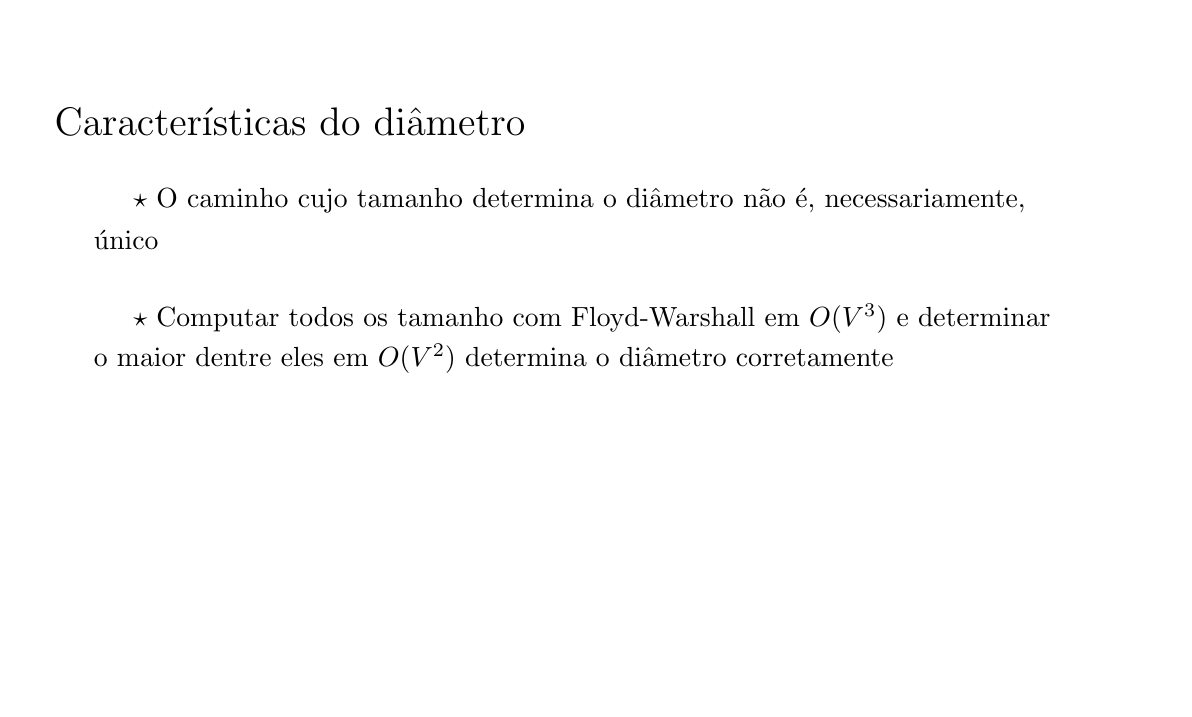
\begin{tikzpicture}
\node[draw,opacity=0] at (0, 0) {x};
\node[draw,opacity=0] at (14, 8) {x};

	\node[anchor=west] (title) at (0.0, 7.0) { \Large \bbbold{Características do diâmetro} };


	\node[anchor=west] (a) at (1.0, 6.0) { $\star$ \bbtext{O caminho cujo tamanho determina o diâmetro não é, necessariamente, } };

	\node[anchor=west] (a1) at (0.5, 5.5) { \bbtext{único} };


	\node[anchor=west] (b) at (1.0, 4.5) { $\star$ \bbtext{Computar todos os tamanho com Floyd-Warshall em $O(V^3)$ e determinar} };

	\node[anchor=west] (b1) at (0.5, 4.0) { \bbtext{o maior dentre eles em $O(V^2)$ determina o diâmetro corretamente} };

\end{tikzpicture}
\end{frame}
\begin{frame}[plain,t]
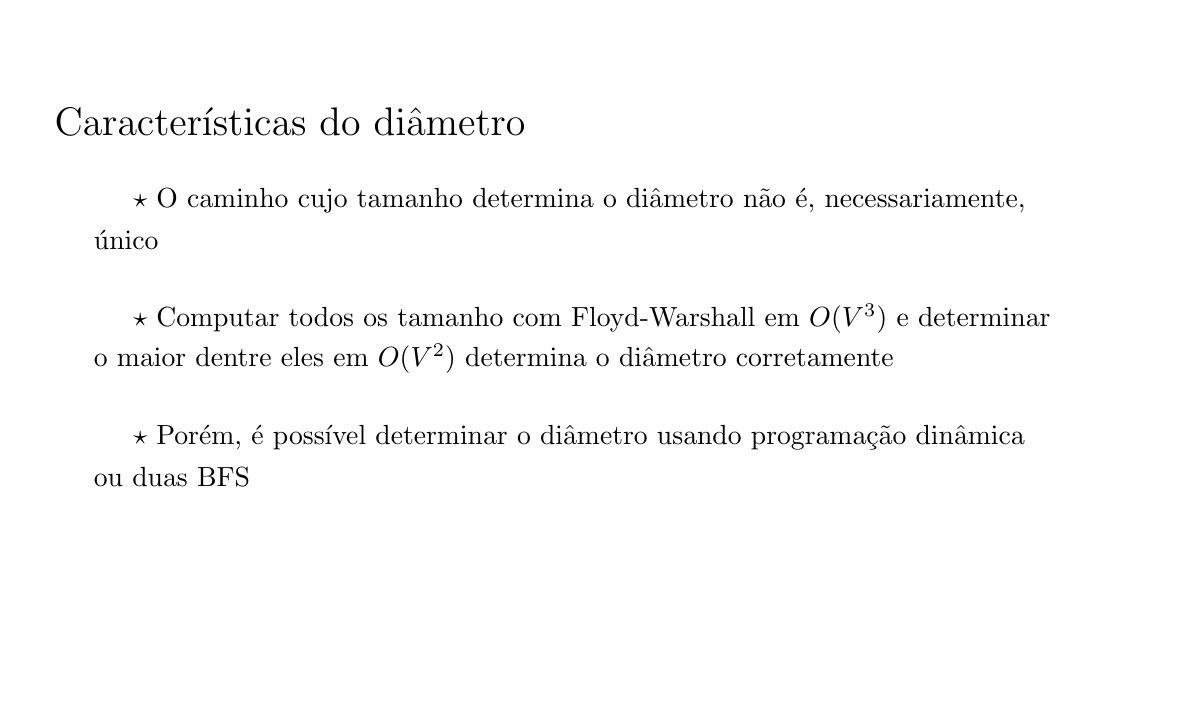
\begin{tikzpicture}
\node[draw,opacity=0] at (0, 0) {x};
\node[draw,opacity=0] at (14, 8) {x};

	\node[anchor=west] (title) at (0.0, 7.0) { \Large \bbbold{Características do diâmetro} };


	\node[anchor=west] (a) at (1.0, 6.0) { $\star$ \bbtext{O caminho cujo tamanho determina o diâmetro não é, necessariamente, } };

	\node[anchor=west] (a1) at (0.5, 5.5) { \bbtext{único} };


	\node[anchor=west] (b) at (1.0, 4.5) { $\star$ \bbtext{Computar todos os tamanho com Floyd-Warshall em $O(V^3)$ e determinar} };

	\node[anchor=west] (b1) at (0.5, 4.0) { \bbtext{o maior dentre eles em $O(V^2)$ determina o diâmetro corretamente} };


	\node[anchor=west] (c) at (1.0, 3.0) { $\star$ \bbtext{Porém, é possível determinar o diâmetro usando programação dinâmica} };

	\node[anchor=west] (c1) at (0.5, 2.5) { \bbtext{ou duas BFS} };

\end{tikzpicture}
\end{frame}
\begin{frame}[plain,t]
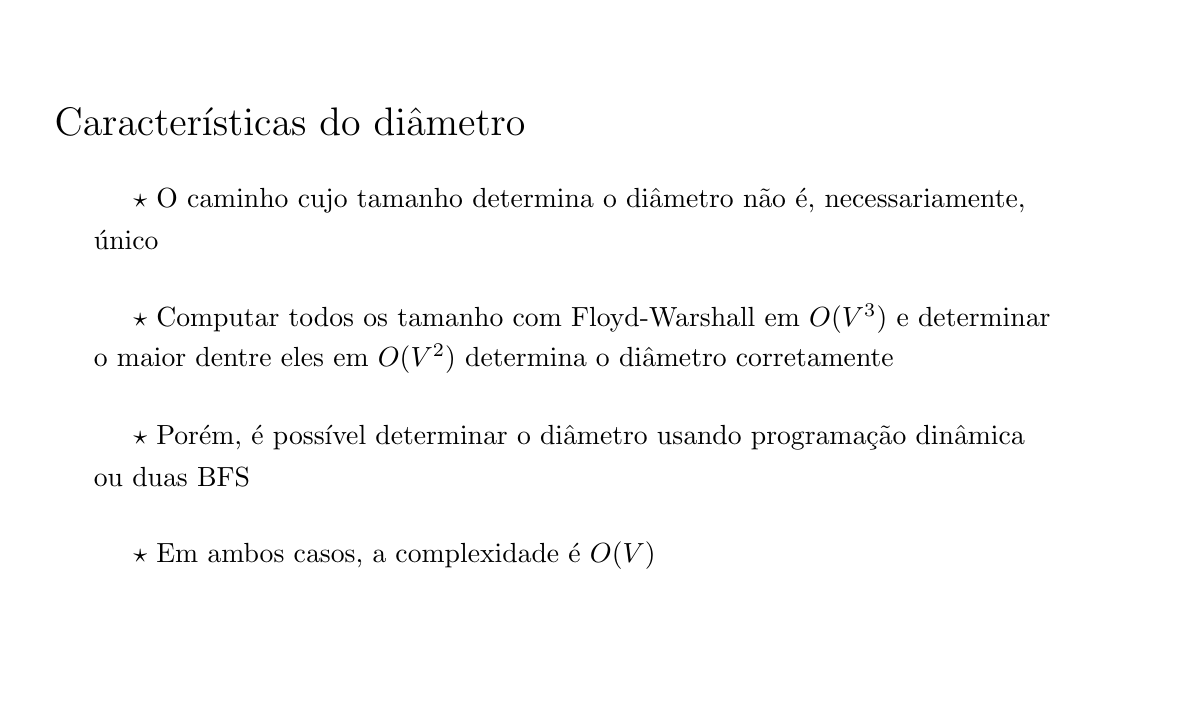
\begin{tikzpicture}
\node[draw,opacity=0] at (0, 0) {x};
\node[draw,opacity=0] at (14, 8) {x};

	\node[anchor=west] (title) at (0.0, 7.0) { \Large \bbbold{Características do diâmetro} };


	\node[anchor=west] (a) at (1.0, 6.0) { $\star$ \bbtext{O caminho cujo tamanho determina o diâmetro não é, necessariamente, } };

	\node[anchor=west] (a1) at (0.5, 5.5) { \bbtext{único} };


	\node[anchor=west] (b) at (1.0, 4.5) { $\star$ \bbtext{Computar todos os tamanho com Floyd-Warshall em $O(V^3)$ e determinar} };

	\node[anchor=west] (b1) at (0.5, 4.0) { \bbtext{o maior dentre eles em $O(V^2)$ determina o diâmetro corretamente} };


	\node[anchor=west] (c) at (1.0, 3.0) { $\star$ \bbtext{Porém, é possível determinar o diâmetro usando programação dinâmica} };

	\node[anchor=west] (c1) at (0.5, 2.5) { \bbtext{ou duas BFS} };


	\node[anchor=west] (d) at (1.0, 1.5) { $\star$ \bbtext{Em ambos casos, a complexidade é $O(V)$} };

\end{tikzpicture}
\end{frame}
\begin{frame}[plain,t]
\begin{tikzpicture}
\node[draw,opacity=0] at (0, 0) {x};
\node[draw,opacity=0] at (14, 8) {x};

	\node[draw,very thick,circle] (node1) at (1.0, 1.0) { \bbtext{1} };

	\node[draw,very thick,circle] (node2) at (7.0, 2.0) { \bbtext{2} };

	\node[draw,very thick,circle] (node3) at (1.0, 5.0) { \bbtext{3} };

	\node[draw,very thick,circle] (node4) at (7.0, 4.0) { \bbtext{4} };

	\node[draw,very thick,circle] (node5) at (10.0, 6.0) { \bbtext{5} };

	\node[draw,very thick,circle] (node6) at (13.0, 3.0) { \bbtext{6} };

	\node[draw,very thick,circle] (node7) at (4.0, 3.0) { \bbtext{7} };

	\draw[thick](node1) to (node7);

	\draw[thick](node3) to (node7);

	\draw[thick](node4) to (node7);

	\draw[thick](node4) to (node2);

	\draw[thick](node4) to (node5);

	\draw[thick](node6) to (node5);

\end{tikzpicture}
\end{frame}
\begin{frame}[plain,t]
\begin{tikzpicture}
\node[draw,opacity=0] at (0, 0) {x};
\node[draw,opacity=0] at (14, 8) {x};

	\node[draw,very thick,circle] (node1) at (1.0, 1.0) { \bbtext{1} };

	\node[draw,very thick,circle] (node2) at (7.0, 2.0) { \bbtext{2} };

	\node[draw,very thick,circle] (node3) at (1.0, 5.0) { \bbtext{3} };

	\node[draw,very thick,circle] (node4) at (7.0, 4.0) { \bbtext{4} };

	\node[draw,very thick,circle] (node5) at (10.0, 6.0) { \bbtext{5} };

	\node[draw,very thick,circle] (node6) at (13.0, 3.0) { \bbtext{6} };

	\node[draw,very thick,circle] (node7) at (4.0, 3.0) { \bbtext{7} };

	\draw[thick,very thick,color=BBOrange](node1) to (node7);

	\draw[thick](node3) to (node7);

	\draw[thick,very thick,color=BBOrange](node4) to (node7);

	\draw[thick](node4) to (node2);

	\draw[thick,very thick,color=BBOrange](node4) to (node5);

	\draw[thick,very thick,color=BBOrange](node6) to (node5);




	\node[anchor=west] (info) at (2.0, 7.0) { \bbtext{Diâmetro: $4$} };

\end{tikzpicture}
\end{frame}
\begin{frame}[plain,t]
\begin{tikzpicture}
\node[draw,opacity=0] at (0, 0) {x};
\node[draw,opacity=0] at (14, 8) {x};

	\node[anchor=west] (title) at (0.0, 7.0) { \Large \bbbold{Definição de pico de um caminho} };
\end{tikzpicture}
\end{frame}
\begin{frame}[plain,t]
\begin{tikzpicture}
\node[draw,opacity=0] at (0, 0) {x};
\node[draw,opacity=0] at (14, 8) {x};

	\node[anchor=west] (title) at (0.0, 7.0) { \Large \bbbold{Definição de pico de um caminho} };

	\node[anchor=west] (a) at (1.0, 6.0) { \bbtext{Seja $T$ uma árvore enraizada e considere dois vértices $u$ e $v$ de $T$. O pico do} };

	\node[anchor=west] (b) at (0.5, 5.25) { \bbtext{caminho de $u$ a $v$ é o nó que ocupa o nível mais baixo em $T$.} };

\end{tikzpicture}
\end{frame}
\begin{frame}[plain,t]
\begin{tikzpicture}
\node[draw,opacity=0] at (0, 0) {x};
\node[draw,opacity=0] at (14, 8) {x};

	\node[anchor=west] (title) at (0.0, 7.0) { \Large \bbbold{Definição de pico de um caminho} };

	\node[anchor=west] (a) at (1.0, 6.0) { \bbtext{Seja $T$ uma árvore enraizada e considere dois vértices $u$ e $v$ de $T$. O pico do} };

	\node[anchor=west] (b) at (0.5, 5.25) { \bbtext{caminho de $u$ a $v$ é o nó que ocupa o nível mais baixo em $T$.} };


	\node[draw,thick,circle] (nodeA) at (9.0, 4.0) { \tiny $a$ };

	\node[draw,thick,circle] (nodeB) at (6.0, 3.0) { \tiny $b$ };

	\node[draw,thick,circle] (nodeC) at (10.0, 3.0) { \tiny $c$ };

	\node[draw,thick,circle] (nodeD) at (4.0, 2.0) { \tiny $d$ };

	\node[draw,thick,circle] (nodeE) at (3.0, 1.0) { \tiny $e$ };

	\node[draw,thick,circle] (nodeG) at (7.0, 1.0) { \tiny $g$ };

	\node[fill=BBGreen,draw,thick,circle] (nodeU) at (5.0, 1.0) { \tiny $\textcolor{BBWhite}{u}$ };

	\node[fill=BBCyan,draw,thick,circle] (nodeV) at (8.0, 2.0) { \tiny $\textcolor{BBWhite}{v}$ };

	\draw[thick](nodeA) to (nodeB);

	\draw[thick](nodeA) to (nodeC);

	\draw[thick](nodeD) to (nodeB);

	\draw[thick](nodeV) to (nodeB);

	\draw[thick](nodeD) to (nodeE);

	\draw[thick](nodeD) to (nodeU);

	\draw[thick](nodeV) to (nodeG);

\end{tikzpicture}
\end{frame}
\begin{frame}[plain,t]
\begin{tikzpicture}
\node[draw,opacity=0] at (0, 0) {x};
\node[draw,opacity=0] at (14, 8) {x};

	\node[anchor=west] (title) at (0.0, 7.0) { \Large \bbbold{Definição de pico de um caminho} };

	\node[anchor=west] (a) at (1.0, 6.0) { \bbtext{Seja $T$ uma árvore enraizada e considere dois vértices $u$ e $v$ de $T$. O pico do} };

	\node[anchor=west] (b) at (0.5, 5.25) { \bbtext{caminho de $u$ a $v$ é o nó que ocupa o nível mais baixo em $T$.} };


	\node[draw,thick,circle] (nodeA) at (9.0, 4.0) { \tiny $a$ };

	\node[draw,thick,circle] (nodeB) at (6.0, 3.0) { \tiny $b$ };

	\node[draw,thick,circle] (nodeC) at (10.0, 3.0) { \tiny $c$ };

	\node[draw,thick,circle] (nodeD) at (4.0, 2.0) { \tiny $d$ };

	\node[draw,thick,circle] (nodeE) at (3.0, 1.0) { \tiny $e$ };

	\node[draw,thick,circle] (nodeG) at (7.0, 1.0) { \tiny $g$ };

	\node[fill=BBGreen,draw,thick,circle] (nodeU) at (5.0, 1.0) { \tiny $\textcolor{BBWhite}{u}$ };

	\node[fill=BBCyan,draw,thick,circle] (nodeV) at (8.0, 2.0) { \tiny $\textcolor{BBWhite}{v}$ };

	\draw[thick](nodeA) to (nodeB);

	\draw[thick](nodeA) to (nodeC);

	\draw[thick,dashed](nodeD) to (nodeB);

	\draw[thick,dashed](nodeV) to (nodeB);

	\draw[thick](nodeD) to (nodeE);

	\draw[thick,dashed](nodeD) to (nodeU);

	\draw[thick](nodeV) to (nodeG);


\end{tikzpicture}
\end{frame}
\begin{frame}[plain,t]
\begin{tikzpicture}
\node[draw,opacity=0] at (0, 0) {x};
\node[draw,opacity=0] at (14, 8) {x};

	\node[anchor=west] (title) at (0.0, 7.0) { \Large \bbbold{Definição de pico de um caminho} };

	\node[anchor=west] (a) at (1.0, 6.0) { \bbtext{Seja $T$ uma árvore enraizada e considere dois vértices $u$ e $v$ de $T$. O pico do} };

	\node[anchor=west] (b) at (0.5, 5.25) { \bbtext{caminho de $u$ a $v$ é o nó que ocupa o nível mais baixo em $T$.} };


	\node[draw,thick,circle] (nodeA) at (9.0, 4.0) { \tiny $a$ };

	\node[draw,thick,circle,fill=BBOrange] (nodeB) at (6.0, 3.0) { \tiny $\textcolor{BBWhite}{b}$ };

	\node[draw,thick,circle] (nodeC) at (10.0, 3.0) { \tiny $c$ };

	\node[draw,thick,circle] (nodeD) at (4.0, 2.0) { \tiny $d$ };

	\node[draw,thick,circle] (nodeE) at (3.0, 1.0) { \tiny $e$ };

	\node[draw,thick,circle] (nodeG) at (7.0, 1.0) { \tiny $g$ };

	\node[fill=BBGreen,draw,thick,circle] (nodeU) at (5.0, 1.0) { \tiny $\textcolor{BBWhite}{u}$ };

	\node[fill=BBCyan,draw,thick,circle] (nodeV) at (8.0, 2.0) { \tiny $\textcolor{BBWhite}{v}$ };

	\draw[thick](nodeA) to (nodeB);

	\draw[thick](nodeA) to (nodeC);

	\draw[thick,dashed](nodeD) to (nodeB);

	\draw[thick,dashed](nodeV) to (nodeB);

	\draw[thick](nodeD) to (nodeE);

	\draw[thick,dashed](nodeD) to (nodeU);

	\draw[thick](nodeV) to (nodeG);



	\draw[color=BBViolet,-latex] (5.0, 3.5) to [bend left]  (5.7, 3.3);

	\node[anchor=east] (info) at (5.0, 3.5) { \scriptsize \bbcomment{pico} };

\end{tikzpicture}
\end{frame}
\begin{frame}[plain,t]
\begin{tikzpicture}
\node[draw,opacity=0] at (0, 0) {x};
\node[draw,opacity=0] at (14, 8) {x};

	\node[anchor=west] (title) at (0.0, 6.0) { \Large \bbbold{Diâmetro de uma árvore com programação dinâmica} };
\end{tikzpicture}
\end{frame}
\begin{frame}[plain,t]
\begin{tikzpicture}
\node[draw,opacity=0] at (0, 0) {x};
\node[draw,opacity=0] at (14, 8) {x};

	\node[anchor=west] (title) at (0.0, 6.0) { \Large \bbbold{Diâmetro de uma árvore com programação dinâmica} };

	\node[anchor=west] (a) at (2.0, 3.0) { $\displaystyle \mathrm{maxLength}[u]$ };

\end{tikzpicture}
\end{frame}
\begin{frame}[plain,t]
\begin{tikzpicture}
\node[draw,opacity=0] at (0, 0) {x};
\node[draw,opacity=0] at (14, 8) {x};

	\node[anchor=west] (title) at (0.0, 6.0) { \Large \bbbold{Diâmetro de uma árvore com programação dinâmica} };

	\node[anchor=west] (a) at (2.0, 3.0) { $\displaystyle \mathrm{maxLength}[u]$ };


	\node[anchor=west] (info) at (1.0, 4.6) { \footnotesize \bbcomment{Tamanho do maior caminho que tem pico igual a $u$} };

	\draw[color=BBViolet,-latex] (3.0, 3.3) to  (3.0, 4.3);

\end{tikzpicture}
\end{frame}
\begin{frame}[plain,t]
\begin{tikzpicture}
\node[draw,opacity=0] at (0, 0) {x};
\node[draw,opacity=0] at (14, 8) {x};

	\node[anchor=west] (title) at (0.0, 6.0) { \Large \bbbold{Diâmetro de uma árvore com programação dinâmica} };

	\node[anchor=west] (a) at (2.0, 3.0) { $\displaystyle \mathrm{maxLength}[u] = \left\{ \begin{array}{ll} 0,& \mbox{se $u$ não tem filhos}\\ \ \\ \end{array}\right.$ };






\end{tikzpicture}
\end{frame}
\begin{frame}[plain,t]
\begin{tikzpicture}
\node[draw,opacity=0] at (0, 0) {x};
\node[draw,opacity=0] at (14, 8) {x};

	\node[anchor=west] (title) at (0.0, 6.0) { \Large \bbbold{Diâmetro de uma árvore com programação dinâmica} };

	\node[anchor=west] (a) at (2.0, 3.0) { $\displaystyle \mathrm{maxLength}[u] = \left\{ \begin{array}{ll} 0,& \mbox{se $u$ não tem filhos}\\ 1 + \mathrm{toLeaf}[v],& \mbox{se $u$ tem apenas um filho $v$}, \\\ \\ \end{array}\right.$ };







\end{tikzpicture}
\end{frame}
\begin{frame}[plain,t]
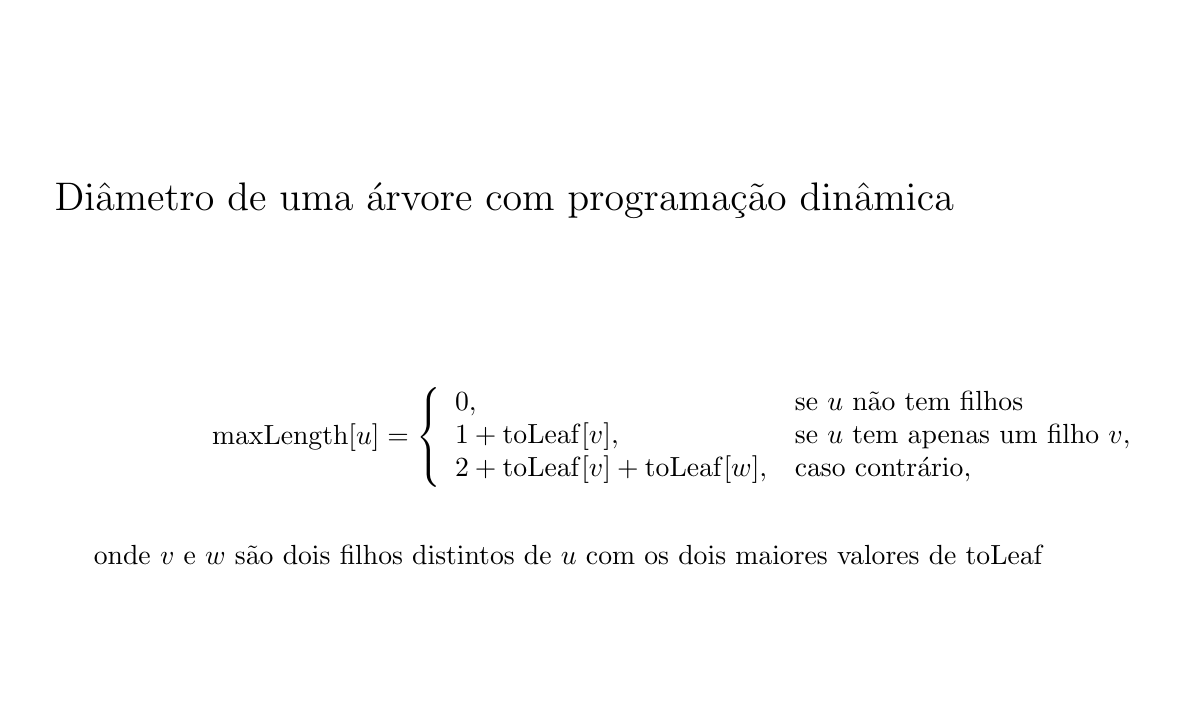
\begin{tikzpicture}
\node[draw,opacity=0] at (0, 0) {x};
\node[draw,opacity=0] at (14, 8) {x};

	\node[anchor=west] (title) at (0.0, 6.0) { \Large \bbbold{Diâmetro de uma árvore com programação dinâmica} };

	\node[anchor=west] (a) at (2.0, 3.0) { $\displaystyle \mathrm{maxLength}[u] = \left\{ \begin{array}{ll} 0,& \mbox{se $u$ não tem filhos}\\ 1 + \mathrm{toLeaf}[v],& \mbox{se $u$ tem apenas um filho $v$}, \\2 + \mathrm{toLeaf}[v] + \mathrm{toLeaf}[w],& \mbox{caso contrário}, \\ \end{array}\right.$ };


	\node[anchor=west] (info) at (0.5, 1.5) { \bbtext{onde $v$ e $w$ são dois filhos distintos de $u$ com os dois maiores valores de $\mathrm{toLeaf}$} };







\end{tikzpicture}
\end{frame}
\begin{frame}[plain,t]
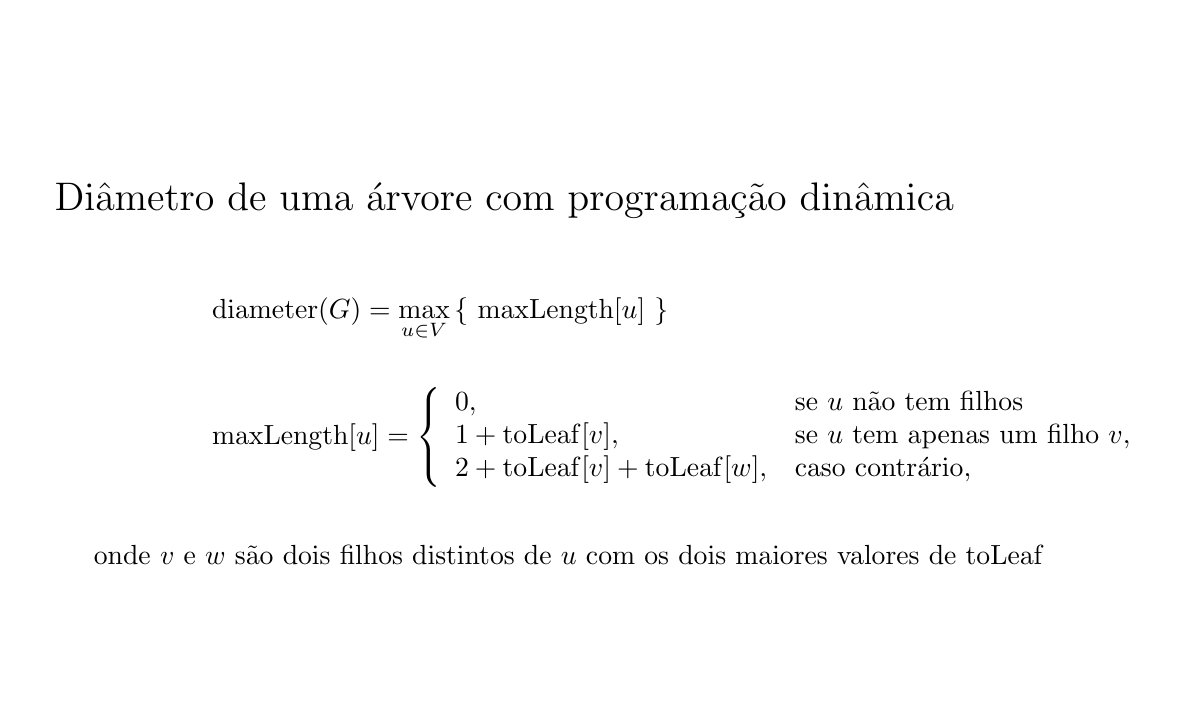
\begin{tikzpicture}
\node[draw,opacity=0] at (0, 0) {x};
\node[draw,opacity=0] at (14, 8) {x};

	\node[anchor=west] (title) at (0.0, 6.0) { \Large \bbbold{Diâmetro de uma árvore com programação dinâmica} };

	\node[anchor=west] (a) at (2.0, 3.0) { $\displaystyle \mathrm{maxLength}[u] = \left\{ \begin{array}{ll} 0,& \mbox{se $u$ não tem filhos}\\ 1 + \mathrm{toLeaf}[v],& \mbox{se $u$ tem apenas um filho $v$}, \\2 + \mathrm{toLeaf}[v] + \mathrm{toLeaf}[w],& \mbox{caso contrário}, \\ \end{array}\right.$ };


	\node[anchor=west] (info) at (0.5, 1.5) { \bbtext{onde $v$ e $w$ são dois filhos distintos de $u$ com os dois maiores valores de $\mathrm{toLeaf}$} };








	\node[anchor=west] (diameter) at (2.0, 4.5) { $\displaystyle \mathrm{diameter}(G) = \max_{u\in V} \left\{\ \mathrm{maxLength}[u]\ \right\}$ };


\end{tikzpicture}
\end{frame}
\begin{frame}[plain,t]
\begin{tikzpicture}
\node[draw,opacity=0] at (0, 0) {x};
\node[draw,opacity=0] at (14, 8) {x};

	\node[draw,very thick,circle] (node4) at (7.0, 7.5) { \bbtext{4} };

	\node[draw,very thick,circle] (node7) at (3.0, 5.5) { \bbtext{7} };

	\node[draw,very thick,circle] (node2) at (7.0, 5.5) { \bbtext{2} };

	\node[draw,very thick,circle] (node5) at (11.0, 5.5) { \bbtext{5} };

	\node[draw,very thick,circle] (node1) at (1.0, 3.5) { \bbtext{1} };

	\node[draw,very thick,circle] (node3) at (5.0, 3.5) { \bbtext{3} };

	\node[draw,very thick,circle] (node6) at (11.0, 3.5) { \bbtext{6} };

	\draw[thick](node4) to (node7);

	\draw[thick](node4) to (node2);

	\draw[thick](node4) to (node5);

	\draw[thick](node7) to (node1);

	\draw[thick](node7) to (node3);

	\draw[thick](node5) to (node6);

	\draw[] (4.0, 0.0) grid  (11.0, 1.0);

	\draw[] (4.0, 1.0) grid  (11.0, 2.0);

	\node[anchor=east] (text) at (3.9, 0.5) { $\mathrm{maxLength}[u] = $ };

	\node[anchor=east] (text2) at (3.9, 1.5) { $\mathrm{toLeaf}[u] = $ };

	\node[] (1) at (4.5, 2.5) { \bbtext{1} };

	\node[] (2) at (5.5, 2.5) { \bbtext{2} };

	\node[] (3) at (6.5, 2.5) { \bbtext{3} };

	\node[] (4) at (7.5, 2.5) { \bbtext{4} };

	\node[] (5) at (8.5, 2.5) { \bbtext{5} };

	\node[] (6) at (9.5, 2.5) { \bbtext{6} };

	\node[] (7) at (10.5, 2.5) { \bbtext{7} };

	\node[] (n1) at (4.5, 0.5) { \bbtext{-} };

	\node[] (n2) at (5.5, 0.5) { \bbtext{-} };

	\node[] (n3) at (6.5, 0.5) { \bbtext{-} };

	\node[] (n4) at (7.5, 0.5) { \bbtext{-} };

	\node[] (n5) at (8.5, 0.5) { \bbtext{-} };

	\node[] (n6) at (9.5, 0.5) { \bbtext{-} };

	\node[] (n7) at (10.5, 0.5) { \bbtext{-} };

	\node[] (L1) at (4.5, 1.5) { \bbtext{-} };

	\node[] (L2) at (5.5, 1.5) { \bbtext{-} };

	\node[] (L3) at (6.5, 1.5) { \bbtext{-} };

	\node[] (L4) at (7.5, 1.5) { \bbtext{-} };

	\node[] (L5) at (8.5, 1.5) { \bbtext{-} };

	\node[] (L6) at (9.5, 1.5) { \bbtext{-} };

	\node[] (L7) at (10.5, 1.5) { \bbtext{-} };

\end{tikzpicture}
\end{frame}
\begin{frame}[plain,t]
\begin{tikzpicture}
\node[draw,opacity=0] at (0, 0) {x};
\node[draw,opacity=0] at (14, 8) {x};

	\node[draw,very thick,circle] (node4) at (7.0, 7.5) { \bbtext{4} };

	\node[draw,very thick,circle] (node7) at (3.0, 5.5) { \bbtext{7} };

	\node[draw,very thick,circle] (node2) at (7.0, 5.5) { \bbtext{2} };

	\node[draw,very thick,circle] (node5) at (11.0, 5.5) { \bbtext{5} };

	\node[draw,very thick,circle,fill=BBCyan] (node1) at (1.0, 3.5) { \bbtext{1} };

	\node[draw,very thick,circle] (node3) at (5.0, 3.5) { \bbtext{3} };

	\node[draw,very thick,circle] (node6) at (11.0, 3.5) { \bbtext{6} };

	\draw[thick](node4) to (node7);

	\draw[thick](node4) to (node2);

	\draw[thick](node4) to (node5);

	\draw[thick](node7) to (node1);

	\draw[thick](node7) to (node3);

	\draw[thick](node5) to (node6);

	\draw[] (4.0, 0.0) grid  (11.0, 1.0);

	\draw[] (4.0, 1.0) grid  (11.0, 2.0);

	\node[anchor=east] (text) at (3.9, 0.5) { $\mathrm{maxLength}[u] = $ };

	\node[anchor=east] (text2) at (3.9, 1.5) { $\mathrm{toLeaf}[u] = $ };

	\node[] (1) at (4.5, 2.5) { \bbtext{1} };

	\node[] (2) at (5.5, 2.5) { \bbtext{2} };

	\node[] (3) at (6.5, 2.5) { \bbtext{3} };

	\node[] (4) at (7.5, 2.5) { \bbtext{4} };

	\node[] (5) at (8.5, 2.5) { \bbtext{5} };

	\node[] (6) at (9.5, 2.5) { \bbtext{6} };

	\node[] (7) at (10.5, 2.5) { \bbtext{7} };

	\node[] (n1) at (4.5, 0.5) { $\mathbf{0}$ };

	\node[] (n2) at (5.5, 0.5) { \bbtext{-} };

	\node[] (n3) at (6.5, 0.5) { \bbtext{-} };

	\node[] (n4) at (7.5, 0.5) { \bbtext{-} };

	\node[] (n5) at (8.5, 0.5) { \bbtext{-} };

	\node[] (n6) at (9.5, 0.5) { \bbtext{-} };

	\node[] (n7) at (10.5, 0.5) { \bbtext{-} };

	\node[] (L1) at (4.5, 1.5) { $\mathbf{0}$ };

	\node[] (L2) at (5.5, 1.5) { \bbtext{-} };

	\node[] (L3) at (6.5, 1.5) { \bbtext{-} };

	\node[] (L4) at (7.5, 1.5) { \bbtext{-} };

	\node[] (L5) at (8.5, 1.5) { \bbtext{-} };

	\node[] (L6) at (9.5, 1.5) { \bbtext{-} };

	\node[] (L7) at (10.5, 1.5) { \bbtext{-} };


\end{tikzpicture}
\end{frame}
\begin{frame}[plain,t]
\begin{tikzpicture}
\node[draw,opacity=0] at (0, 0) {x};
\node[draw,opacity=0] at (14, 8) {x};

	\node[draw,very thick,circle] (node4) at (7.0, 7.5) { \bbtext{4} };

	\node[draw,very thick,circle] (node7) at (3.0, 5.5) { \bbtext{7} };

	\node[draw,very thick,circle] (node2) at (7.0, 5.5) { \bbtext{2} };

	\node[draw,very thick,circle] (node5) at (11.0, 5.5) { \bbtext{5} };

	\node[draw,very thick,circle,fill=BBCyan] (node1) at (1.0, 3.5) { \bbtext{1} };

	\node[draw,very thick,circle,fill=BBCyan] (node3) at (5.0, 3.5) { \bbtext{3} };

	\node[draw,very thick,circle] (node6) at (11.0, 3.5) { \bbtext{6} };

	\draw[thick](node4) to (node7);

	\draw[thick](node4) to (node2);

	\draw[thick](node4) to (node5);

	\draw[thick](node7) to (node1);

	\draw[thick](node7) to (node3);

	\draw[thick](node5) to (node6);

	\draw[] (4.0, 0.0) grid  (11.0, 1.0);

	\draw[] (4.0, 1.0) grid  (11.0, 2.0);

	\node[anchor=east] (text) at (3.9, 0.5) { $\mathrm{maxLength}[u] = $ };

	\node[anchor=east] (text2) at (3.9, 1.5) { $\mathrm{toLeaf}[u] = $ };

	\node[] (1) at (4.5, 2.5) { \bbtext{1} };

	\node[] (2) at (5.5, 2.5) { \bbtext{2} };

	\node[] (3) at (6.5, 2.5) { \bbtext{3} };

	\node[] (4) at (7.5, 2.5) { \bbtext{4} };

	\node[] (5) at (8.5, 2.5) { \bbtext{5} };

	\node[] (6) at (9.5, 2.5) { \bbtext{6} };

	\node[] (7) at (10.5, 2.5) { \bbtext{7} };

	\node[] (n1) at (4.5, 0.5) { ${0}$ };

	\node[] (n2) at (5.5, 0.5) { \bbtext{-} };

	\node[] (n3) at (6.5, 0.5) { $\mathbf{0}$ };

	\node[] (n4) at (7.5, 0.5) { \bbtext{-} };

	\node[] (n5) at (8.5, 0.5) { \bbtext{-} };

	\node[] (n6) at (9.5, 0.5) { \bbtext{-} };

	\node[] (n7) at (10.5, 0.5) { \bbtext{-} };

	\node[] (L1) at (4.5, 1.5) { ${0}$ };

	\node[] (L2) at (5.5, 1.5) { \bbtext{-} };

	\node[] (L3) at (6.5, 1.5) { $\mathbf{0}$ };

	\node[] (L4) at (7.5, 1.5) { \bbtext{-} };

	\node[] (L5) at (8.5, 1.5) { \bbtext{-} };

	\node[] (L6) at (9.5, 1.5) { \bbtext{-} };

	\node[] (L7) at (10.5, 1.5) { \bbtext{-} };



\end{tikzpicture}
\end{frame}
\begin{frame}[plain,t]
\begin{tikzpicture}
\node[draw,opacity=0] at (0, 0) {x};
\node[draw,opacity=0] at (14, 8) {x};

	\node[draw,very thick,circle] (node4) at (7.0, 7.5) { \bbtext{4} };

	\node[draw,very thick,circle] (node7) at (3.0, 5.5) { \bbtext{7} };

	\node[draw,very thick,circle,fill=BBCyan] (node2) at (7.0, 5.5) { \bbtext{2} };

	\node[draw,very thick,circle] (node5) at (11.0, 5.5) { \bbtext{5} };

	\node[draw,very thick,circle,fill=BBCyan] (node1) at (1.0, 3.5) { \bbtext{1} };

	\node[draw,very thick,circle,fill=BBCyan] (node3) at (5.0, 3.5) { \bbtext{3} };

	\node[draw,very thick,circle] (node6) at (11.0, 3.5) { \bbtext{6} };

	\draw[thick](node4) to (node7);

	\draw[thick](node4) to (node2);

	\draw[thick](node4) to (node5);

	\draw[thick](node7) to (node1);

	\draw[thick](node7) to (node3);

	\draw[thick](node5) to (node6);

	\draw[] (4.0, 0.0) grid  (11.0, 1.0);

	\draw[] (4.0, 1.0) grid  (11.0, 2.0);

	\node[anchor=east] (text) at (3.9, 0.5) { $\mathrm{maxLength}[u] = $ };

	\node[anchor=east] (text2) at (3.9, 1.5) { $\mathrm{toLeaf}[u] = $ };

	\node[] (1) at (4.5, 2.5) { \bbtext{1} };

	\node[] (2) at (5.5, 2.5) { \bbtext{2} };

	\node[] (3) at (6.5, 2.5) { \bbtext{3} };

	\node[] (4) at (7.5, 2.5) { \bbtext{4} };

	\node[] (5) at (8.5, 2.5) { \bbtext{5} };

	\node[] (6) at (9.5, 2.5) { \bbtext{6} };

	\node[] (7) at (10.5, 2.5) { \bbtext{7} };

	\node[] (n1) at (4.5, 0.5) { ${0}$ };

	\node[] (n2) at (5.5, 0.5) { $\mathbf{0}$ };

	\node[] (n3) at (6.5, 0.5) { ${0}$ };

	\node[] (n4) at (7.5, 0.5) { \bbtext{-} };

	\node[] (n5) at (8.5, 0.5) { \bbtext{-} };

	\node[] (n6) at (9.5, 0.5) { \bbtext{-} };

	\node[] (n7) at (10.5, 0.5) { \bbtext{-} };

	\node[] (L1) at (4.5, 1.5) { ${0}$ };

	\node[] (L2) at (5.5, 1.5) { $\mathbf{0}$ };

	\node[] (L3) at (6.5, 1.5) { ${0}$ };

	\node[] (L4) at (7.5, 1.5) { \bbtext{-} };

	\node[] (L5) at (8.5, 1.5) { \bbtext{-} };

	\node[] (L6) at (9.5, 1.5) { \bbtext{-} };

	\node[] (L7) at (10.5, 1.5) { \bbtext{-} };




\end{tikzpicture}
\end{frame}
\begin{frame}[plain,t]
\begin{tikzpicture}
\node[draw,opacity=0] at (0, 0) {x};
\node[draw,opacity=0] at (14, 8) {x};

	\node[draw,very thick,circle] (node4) at (7.0, 7.5) { \bbtext{4} };

	\node[draw,very thick,circle] (node7) at (3.0, 5.5) { \bbtext{7} };

	\node[draw,very thick,circle,fill=BBCyan] (node2) at (7.0, 5.5) { \bbtext{2} };

	\node[draw,very thick,circle] (node5) at (11.0, 5.5) { \bbtext{5} };

	\node[draw,very thick,circle,fill=BBCyan] (node1) at (1.0, 3.5) { \bbtext{1} };

	\node[draw,very thick,circle,fill=BBCyan] (node3) at (5.0, 3.5) { \bbtext{3} };

	\node[draw,very thick,circle,fill=BBCyan] (node6) at (11.0, 3.5) { \bbtext{6} };

	\draw[thick](node4) to (node7);

	\draw[thick](node4) to (node2);

	\draw[thick](node4) to (node5);

	\draw[thick](node7) to (node1);

	\draw[thick](node7) to (node3);

	\draw[thick](node5) to (node6);

	\draw[] (4.0, 0.0) grid  (11.0, 1.0);

	\draw[] (4.0, 1.0) grid  (11.0, 2.0);

	\node[anchor=east] (text) at (3.9, 0.5) { $\mathrm{maxLength}[u] = $ };

	\node[anchor=east] (text2) at (3.9, 1.5) { $\mathrm{toLeaf}[u] = $ };

	\node[] (1) at (4.5, 2.5) { \bbtext{1} };

	\node[] (2) at (5.5, 2.5) { \bbtext{2} };

	\node[] (3) at (6.5, 2.5) { \bbtext{3} };

	\node[] (4) at (7.5, 2.5) { \bbtext{4} };

	\node[] (5) at (8.5, 2.5) { \bbtext{5} };

	\node[] (6) at (9.5, 2.5) { \bbtext{6} };

	\node[] (7) at (10.5, 2.5) { \bbtext{7} };

	\node[] (n1) at (4.5, 0.5) { ${0}$ };

	\node[] (n2) at (5.5, 0.5) { ${0}$ };

	\node[] (n3) at (6.5, 0.5) { ${0}$ };

	\node[] (n4) at (7.5, 0.5) { \bbtext{-} };

	\node[] (n5) at (8.5, 0.5) { \bbtext{-} };

	\node[] (n6) at (9.5, 0.5) { $\mathbf{0}$ };

	\node[] (n7) at (10.5, 0.5) { \bbtext{-} };

	\node[] (L1) at (4.5, 1.5) { ${0}$ };

	\node[] (L2) at (5.5, 1.5) { ${0}$ };

	\node[] (L3) at (6.5, 1.5) { ${0}$ };

	\node[] (L4) at (7.5, 1.5) { \bbtext{-} };

	\node[] (L5) at (8.5, 1.5) { \bbtext{-} };

	\node[] (L6) at (9.5, 1.5) { $\mathbf{0}$ };

	\node[] (L7) at (10.5, 1.5) { \bbtext{-} };





\end{tikzpicture}
\end{frame}
\begin{frame}[plain,t]
\begin{tikzpicture}
\node[draw,opacity=0] at (0, 0) {x};
\node[draw,opacity=0] at (14, 8) {x};

	\node[draw,very thick,circle] (node4) at (7.0, 7.5) { \bbtext{4} };

	\node[draw,very thick,circle] (node7) at (3.0, 5.5) { \bbtext{7} };

	\node[draw,very thick,circle,fill=BBCyan] (node2) at (7.0, 5.5) { \bbtext{2} };

	\node[draw,very thick,circle,fill=BBGreen] (node5) at (11.0, 5.5) { \bbtext{5} };

	\node[draw,very thick,circle,fill=BBCyan] (node1) at (1.0, 3.5) { \bbtext{1} };

	\node[draw,very thick,circle,fill=BBCyan] (node3) at (5.0, 3.5) { \bbtext{3} };

	\node[draw,very thick,circle,fill=BBCyan] (node6) at (11.0, 3.5) { \bbtext{6} };

	\draw[thick](node4) to (node7);

	\draw[thick](node4) to (node2);

	\draw[thick](node4) to (node5);

	\draw[thick](node7) to (node1);

	\draw[thick](node7) to (node3);

	\draw[thick](node5) to (node6);

	\draw[] (4.0, 0.0) grid  (11.0, 1.0);

	\draw[] (4.0, 1.0) grid  (11.0, 2.0);

	\node[anchor=east] (text) at (3.9, 0.5) { $\mathrm{maxLength}[u] = $ };

	\node[anchor=east] (text2) at (3.9, 1.5) { $\mathrm{toLeaf}[u] = $ };

	\node[] (1) at (4.5, 2.5) { \bbtext{1} };

	\node[] (2) at (5.5, 2.5) { \bbtext{2} };

	\node[] (3) at (6.5, 2.5) { \bbtext{3} };

	\node[] (4) at (7.5, 2.5) { \bbtext{4} };

	\node[] (5) at (8.5, 2.5) { \bbtext{5} };

	\node[] (6) at (9.5, 2.5) { \bbtext{6} };

	\node[] (7) at (10.5, 2.5) { \bbtext{7} };

	\node[] (n1) at (4.5, 0.5) { ${0}$ };

	\node[] (n2) at (5.5, 0.5) { ${0}$ };

	\node[] (n3) at (6.5, 0.5) { ${0}$ };

	\node[] (n4) at (7.5, 0.5) { \bbtext{-} };

	\node[] (n5) at (8.5, 0.5) { $\mathbf{1}$ };

	\node[] (n6) at (9.5, 0.5) { ${0}$ };

	\node[] (n7) at (10.5, 0.5) { \bbtext{-} };

	\node[] (L1) at (4.5, 1.5) { ${0}$ };

	\node[] (L2) at (5.5, 1.5) { ${0}$ };

	\node[] (L3) at (6.5, 1.5) { ${0}$ };

	\node[] (L4) at (7.5, 1.5) { \bbtext{-} };

	\node[] (L5) at (8.5, 1.5) { $\mathbf{1}$ };

	\node[] (L6) at (9.5, 1.5) { ${0}$ };

	\node[] (L7) at (10.5, 1.5) { \bbtext{-} };






\end{tikzpicture}
\end{frame}
\begin{frame}[plain,t]
\begin{tikzpicture}
\node[draw,opacity=0] at (0, 0) {x};
\node[draw,opacity=0] at (14, 8) {x};

	\node[draw,very thick,circle] (node4) at (7.0, 7.5) { \bbtext{4} };

	\node[draw,very thick,circle,fill=BBOrange] (node7) at (3.0, 5.5) { \bbtext{7} };

	\node[draw,very thick,circle,fill=BBCyan] (node2) at (7.0, 5.5) { \bbtext{2} };

	\node[draw,very thick,circle,fill=BBGreen] (node5) at (11.0, 5.5) { \bbtext{5} };

	\node[draw,very thick,circle,fill=BBCyan] (node1) at (1.0, 3.5) { \bbtext{1} };

	\node[draw,very thick,circle,fill=BBCyan] (node3) at (5.0, 3.5) { \bbtext{3} };

	\node[draw,very thick,circle,fill=BBCyan] (node6) at (11.0, 3.5) { \bbtext{6} };

	\draw[thick](node4) to (node7);

	\draw[thick](node4) to (node2);

	\draw[thick](node4) to (node5);

	\draw[thick](node7) to (node1);

	\draw[thick](node7) to (node3);

	\draw[thick](node5) to (node6);

	\draw[] (4.0, 0.0) grid  (11.0, 1.0);

	\draw[] (4.0, 1.0) grid  (11.0, 2.0);

	\node[anchor=east] (text) at (3.9, 0.5) { $\mathrm{maxLength}[u] = $ };

	\node[anchor=east] (text2) at (3.9, 1.5) { $\mathrm{toLeaf}[u] = $ };

	\node[] (1) at (4.5, 2.5) { \bbtext{1} };

	\node[] (2) at (5.5, 2.5) { \bbtext{2} };

	\node[] (3) at (6.5, 2.5) { \bbtext{3} };

	\node[] (4) at (7.5, 2.5) { \bbtext{4} };

	\node[] (5) at (8.5, 2.5) { \bbtext{5} };

	\node[] (6) at (9.5, 2.5) { \bbtext{6} };

	\node[] (7) at (10.5, 2.5) { \bbtext{7} };

	\node[] (n1) at (4.5, 0.5) { ${0}$ };

	\node[] (n2) at (5.5, 0.5) { ${0}$ };

	\node[] (n3) at (6.5, 0.5) { ${0}$ };

	\node[] (n4) at (7.5, 0.5) { \bbtext{-} };

	\node[] (n5) at (8.5, 0.5) { ${1}$ };

	\node[] (n6) at (9.5, 0.5) { ${0}$ };

	\node[] (n7) at (10.5, 0.5) { $\mathbf{2}$ };

	\node[] (L1) at (4.5, 1.5) { ${0}$ };

	\node[] (L2) at (5.5, 1.5) { ${0}$ };

	\node[] (L3) at (6.5, 1.5) { ${0}$ };

	\node[] (L4) at (7.5, 1.5) { \bbtext{-} };

	\node[] (L5) at (8.5, 1.5) { ${1}$ };

	\node[] (L6) at (9.5, 1.5) { ${0}$ };

	\node[] (L7) at (10.5, 1.5) { $\mathbf{1}$ };







\end{tikzpicture}
\end{frame}
\begin{frame}[plain,t]
\begin{tikzpicture}
\node[draw,opacity=0] at (0, 0) {x};
\node[draw,opacity=0] at (14, 8) {x};

	\node[draw,very thick,circle,fill=BBOrange] (node4) at (7.0, 7.5) { \bbtext{4} };

	\node[draw,very thick,circle,fill=BBOrange] (node7) at (3.0, 5.5) { \bbtext{7} };

	\node[draw,very thick,circle,fill=BBCyan] (node2) at (7.0, 5.5) { \bbtext{2} };

	\node[draw,very thick,circle,fill=BBGreen] (node5) at (11.0, 5.5) { \bbtext{5} };

	\node[draw,very thick,circle,fill=BBCyan] (node1) at (1.0, 3.5) { \bbtext{1} };

	\node[draw,very thick,circle,fill=BBCyan] (node3) at (5.0, 3.5) { \bbtext{3} };

	\node[draw,very thick,circle,fill=BBCyan] (node6) at (11.0, 3.5) { \bbtext{6} };

	\draw[thick](node4) to (node7);

	\draw[thick](node4) to (node2);

	\draw[thick](node4) to (node5);

	\draw[thick](node7) to (node1);

	\draw[thick](node7) to (node3);

	\draw[thick](node5) to (node6);

	\draw[] (4.0, 0.0) grid  (11.0, 1.0);

	\draw[] (4.0, 1.0) grid  (11.0, 2.0);

	\node[anchor=east] (text) at (3.9, 0.5) { $\mathrm{maxLength}[u] = $ };

	\node[anchor=east] (text2) at (3.9, 1.5) { $\mathrm{toLeaf}[u] = $ };

	\node[] (1) at (4.5, 2.5) { \bbtext{1} };

	\node[] (2) at (5.5, 2.5) { \bbtext{2} };

	\node[] (3) at (6.5, 2.5) { \bbtext{3} };

	\node[] (4) at (7.5, 2.5) { \bbtext{4} };

	\node[] (5) at (8.5, 2.5) { \bbtext{5} };

	\node[] (6) at (9.5, 2.5) { \bbtext{6} };

	\node[] (7) at (10.5, 2.5) { \bbtext{7} };

	\node[] (n1) at (4.5, 0.5) { ${0}$ };

	\node[] (n2) at (5.5, 0.5) { ${0}$ };

	\node[] (n3) at (6.5, 0.5) { ${0}$ };

	\node[] (n4) at (7.5, 0.5) { $\mathbf{4}$ };

	\node[] (n5) at (8.5, 0.5) { ${1}$ };

	\node[] (n6) at (9.5, 0.5) { ${0}$ };

	\node[] (n7) at (10.5, 0.5) { ${2}$ };

	\node[] (L1) at (4.5, 1.5) { ${0}$ };

	\node[] (L2) at (5.5, 1.5) { ${0}$ };

	\node[] (L3) at (6.5, 1.5) { ${0}$ };

	\node[] (L4) at (7.5, 1.5) { $\mathbf{2}$ };

	\node[] (L5) at (8.5, 1.5) { ${1}$ };

	\node[] (L6) at (9.5, 1.5) { ${0}$ };

	\node[] (L7) at (10.5, 1.5) { ${1}$ };









\end{tikzpicture}
\end{frame}
\begin{frame}[plain,t]

\inputsnippet{cpp}{43}{53}{codes/dp.cpp}

\end{frame}
\begin{frame}[plain,t]

\inputsnippet{cpp}{10}{25}{codes/dp.cpp}

\end{frame}
\begin{frame}[plain,t]

\inputsnippet{cpp}{27}{41}{codes/dp.cpp}

\end{frame}

\begin{frame}[plain,t]
\begin{tikzpicture}
\node[draw,opacity=0] at (0, 0) {x};
\node[draw,opacity=0] at (14, 8) {x};

	\node[anchor=west] (title) at (0.0, 7.0) { \Large \bbbold{Possível simplificação da DFS} };

\end{tikzpicture}
\end{frame}

\begin{frame}[plain,t]
\begin{tikzpicture}
\node[draw,opacity=0] at (0, 0) {x};
\node[draw,opacity=0] at (14, 8) {x};

	\node[anchor=west] (title) at (0.0, 7.0) { \Large \bbbold{Possível simplificação da DFS} };
  \node[anchor=west] (a) at (0.1, 6.0) { $\star$ \bbtext{Partindo da idéia anterior é possível guardar apenas os dois melhores valores. } };

\end{tikzpicture}
\end{frame}


\begin{frame}[plain,t]
\begin{tikzpicture}
\node[draw,opacity=0] at (0, 0) {x};
\node[draw,opacity=0] at (14, 8) {x};

	\node[anchor=west] (title) at (0.0, 7.0) { \Large \bbbold{Possível simplificação da DFS} };
  \node[anchor=west] (a) at (0.1, 6.0) { $\star$ \bbtext{Partindo da idéia anterior é possível guardar apenas os dois melhores valores. } };
  \node[anchor=west] (a) at (0.1, 5.0) { $\star$ \bbtext{Guardaremos em $\displaystyle \mathrm{d1}$ e $\displaystyle \mathrm{d2}$, o maior e segundo maior valor para $\displaystyle \mathrm{to\_leaf}[v]$.} };

\end{tikzpicture}
\end{frame}

\begin{frame}[plain,t]
\begin{tikzpicture}
\node[draw,opacity=0] at (0, 0) {x};
\node[draw,opacity=0] at (14, 8) {x};
	\node[anchor=west] (title) at (0.0, 7.0) { \Large \bbbold{Possível simplificação da DFS} };

  \node[anchor=west] (a) at (0.1, 6.0) { $\star$ \bbtext{ Fazendo com que  $\displaystyle \mathrm{to\_leaf}[u] = max(\displaystyle \mathrm{d1}, \displaystyle \mathrm{d2}) + 1$ tem-se que :}  };

\end{tikzpicture}
\end{frame}

\begin{frame}[plain,t]
\begin{tikzpicture}
\node[draw,opacity=0] at (0, 0) {x};
\node[draw,opacity=0] at (14, 8) {x};
	\node[anchor=west] (title) at (0.0, 7.0) { \Large \bbbold{Possível simplificação da DFS} };

  \node[anchor=west] (a) at (0.1, 6.0) { $\star$ \bbtext{ Fazendo com que  $\displaystyle \mathrm{to\_leaf}[u] = max(\displaystyle \mathrm{d1}, \displaystyle \mathrm{d2}) + 1$ tem-se que :}  };
  \node[anchor=west] (a) at (0.5, 5.5) { $\star$ \bbtext{Se $u$ for uma folha:  $\displaystyle \mathrm{to\_leaf}[u] = max(\displaystyle \mathrm{d1}, \displaystyle \mathrm{d2}) + 1 = -1 + 1= 0$}  };

\end{tikzpicture}
\end{frame}

\begin{frame}[plain,t]
\begin{tikzpicture}
\node[draw,opacity=0] at (0, 0) {x};
\node[draw,opacity=0] at (14, 8) {x};
	\node[anchor=west] (title) at (0.0, 7.0) { \Large \bbbold{Possível simplificação da DFS} };

  \node[anchor=west] (a) at (0.1, 6.0) { $\star$ \bbtext{ Fazendo com que  $\displaystyle \mathrm{to\_leaf}[u] = max(\displaystyle \mathrm{d1}, \displaystyle \mathrm{d2}) + 1$ tem-se que :}  };
  \node[anchor=west] (a) at (0.5, 5.5) { $\star$ \bbtext{Se $u$ for uma folha:  $\displaystyle \mathrm{to\_leaf}[u] = max(\displaystyle \mathrm{d1}, \displaystyle \mathrm{d2}) + 1 = -1 + 1= 0$}  };
  \node[anchor=west] (a) at (0.5, 5.0) { $\star$ \bbtext{Caso contrário o maior valor será somado.}  };

\end{tikzpicture}
\end{frame}

\begin{frame}[plain,t]
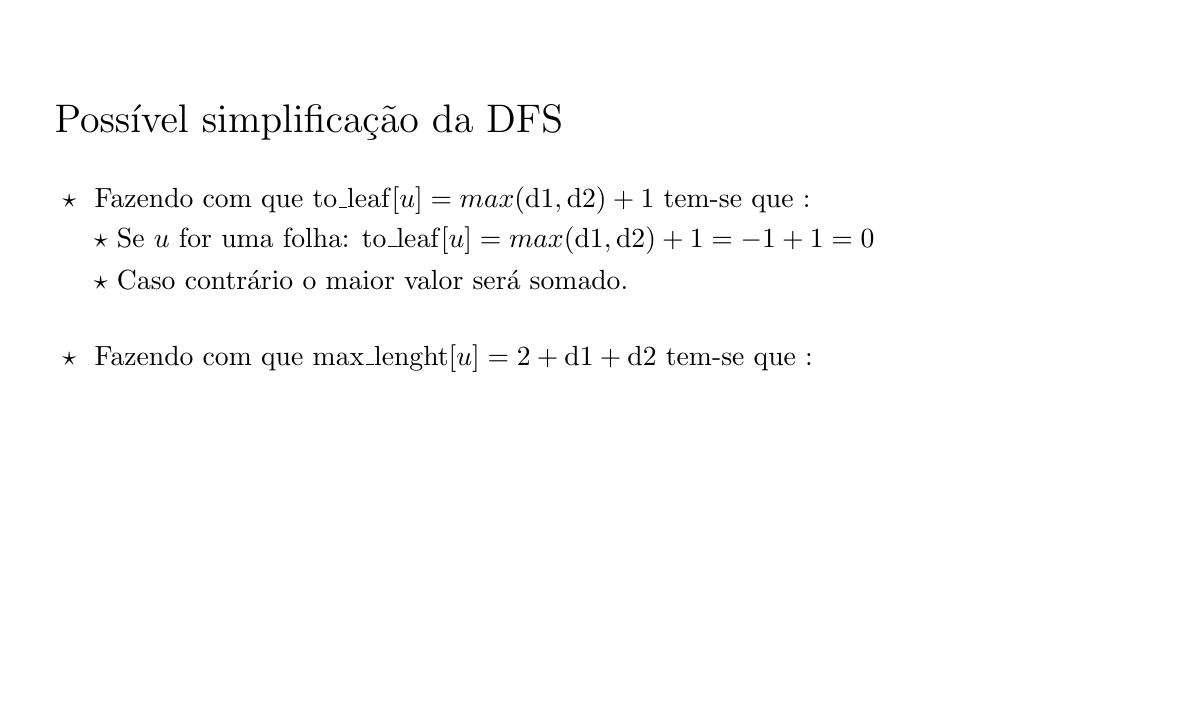
\begin{tikzpicture}
\node[draw,opacity=0] at (0, 0) {x};
\node[draw,opacity=0] at (14, 8) {x};
	\node[anchor=west] (title) at (0.0, 7.0) { \Large \bbbold{Possível simplificação da DFS} };

  \node[anchor=west] (a) at (0.1, 6.0) { $\star$ \bbtext{ Fazendo com que  $\displaystyle \mathrm{to\_leaf}[u] = max(\displaystyle \mathrm{d1}, \displaystyle \mathrm{d2}) + 1$ tem-se que :}  };
  \node[anchor=west] (a) at (0.5, 5.5) { $\star$ \bbtext{Se $u$ for uma folha:  $\displaystyle \mathrm{to\_leaf}[u] = max(\displaystyle \mathrm{d1}, \displaystyle \mathrm{d2}) + 1 = -1 + 1= 0$}  };
  \node[anchor=west] (a) at (0.5, 5.0) { $\star$ \bbtext{Caso contrário o maior valor será somado.}  };


  \node[anchor=west] (a) at (0.1, 4.0) { $\star$ \bbtext{ Fazendo com que  $\displaystyle \mathrm{max\_lenght}[u] = 2 + \displaystyle \mathrm{d1} + \displaystyle \mathrm{d2}$ tem-se que :}  };

\end{tikzpicture}
\end{frame}

\begin{frame}[plain,t]
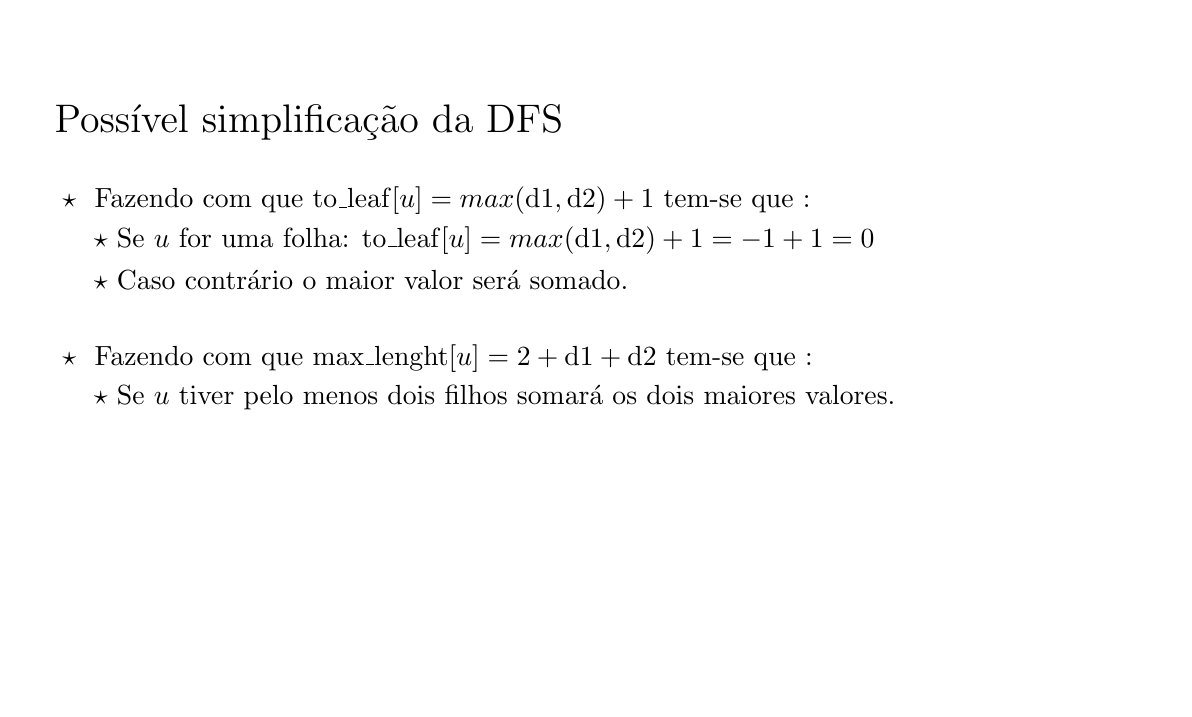
\begin{tikzpicture}
\node[draw,opacity=0] at (0, 0) {x};
\node[draw,opacity=0] at (14, 8) {x};
	\node[anchor=west] (title) at (0.0, 7.0) { \Large \bbbold{Possível simplificação da DFS} };

  \node[anchor=west] (a) at (0.1, 6.0) { $\star$ \bbtext{ Fazendo com que  $\displaystyle \mathrm{to\_leaf}[u] = max(\displaystyle \mathrm{d1}, \displaystyle \mathrm{d2}) + 1$ tem-se que :}  };
  \node[anchor=west] (a) at (0.5, 5.5) { $\star$ \bbtext{Se $u$ for uma folha:  $\displaystyle \mathrm{to\_leaf}[u] = max(\displaystyle \mathrm{d1}, \displaystyle \mathrm{d2}) + 1 = -1 + 1= 0$}  };
  \node[anchor=west] (a) at (0.5, 5.0) { $\star$ \bbtext{Caso contrário o maior valor será somado.}  };


  \node[anchor=west] (a) at (0.1, 4.0) { $\star$ \bbtext{ Fazendo com que  $\displaystyle \mathrm{max\_lenght}[u] = 2 + \displaystyle \mathrm{d1} + \displaystyle \mathrm{d2}$ tem-se que :}  };
  \node[anchor=west] (a) at (0.5, 3.5) { $\star$ \bbtext{Se $u$ tiver pelo menos dois filhos somará os dois maiores valores.}  };

  \end{tikzpicture}
\end{frame}

\begin{frame}[plain,t]
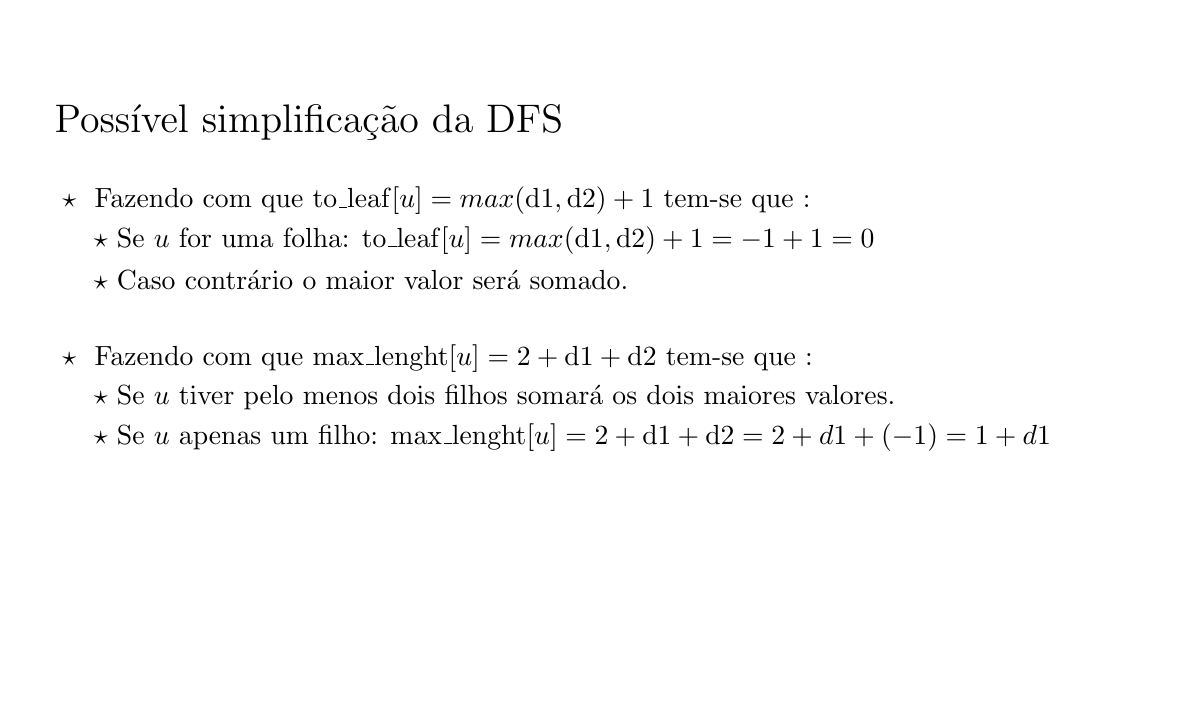
\begin{tikzpicture}
\node[draw,opacity=0] at (0, 0) {x};
\node[draw,opacity=0] at (14, 8) {x};
	\node[anchor=west] (title) at (0.0, 7.0) { \Large \bbbold{Possível simplificação da DFS} };

  \node[anchor=west] (a) at (0.1, 6.0) { $\star$ \bbtext{ Fazendo com que  $\displaystyle \mathrm{to\_leaf}[u] = max(\displaystyle \mathrm{d1}, \displaystyle \mathrm{d2}) + 1$ tem-se que :}  };
  \node[anchor=west] (a) at (0.5, 5.5) { $\star$ \bbtext{Se $u$ for uma folha:  $\displaystyle \mathrm{to\_leaf}[u] = max(\displaystyle \mathrm{d1}, \displaystyle \mathrm{d2}) + 1 = -1 + 1= 0$}  };
  \node[anchor=west] (a) at (0.5, 5.0) { $\star$ \bbtext{Caso contrário o maior valor será somado.}  };


  \node[anchor=west] (a) at (0.1, 4.0) { $\star$ \bbtext{ Fazendo com que  $\displaystyle \mathrm{max\_lenght}[u] = 2 + \displaystyle \mathrm{d1} + \displaystyle \mathrm{d2}$ tem-se que :}  };

  \node[anchor=west] (a) at (0.5, 3.5) { $\star$ \bbtext{Se $u$ tiver pelo menos dois filhos somará os dois maiores valores.}  };
  \node[anchor=west] (a) at (0.5, 3.0) { $\star$ \bbtext{Se $u$ apenas um filho: $\displaystyle \mathrm{max\_lenght}[u] = 2 + \displaystyle \mathrm{d1} + \displaystyle \mathrm{d2} = 2  + d1 + (-1) = 1 + d1$}  };

\end{tikzpicture}
\end{frame}
\begin{frame}[plain,t]
	
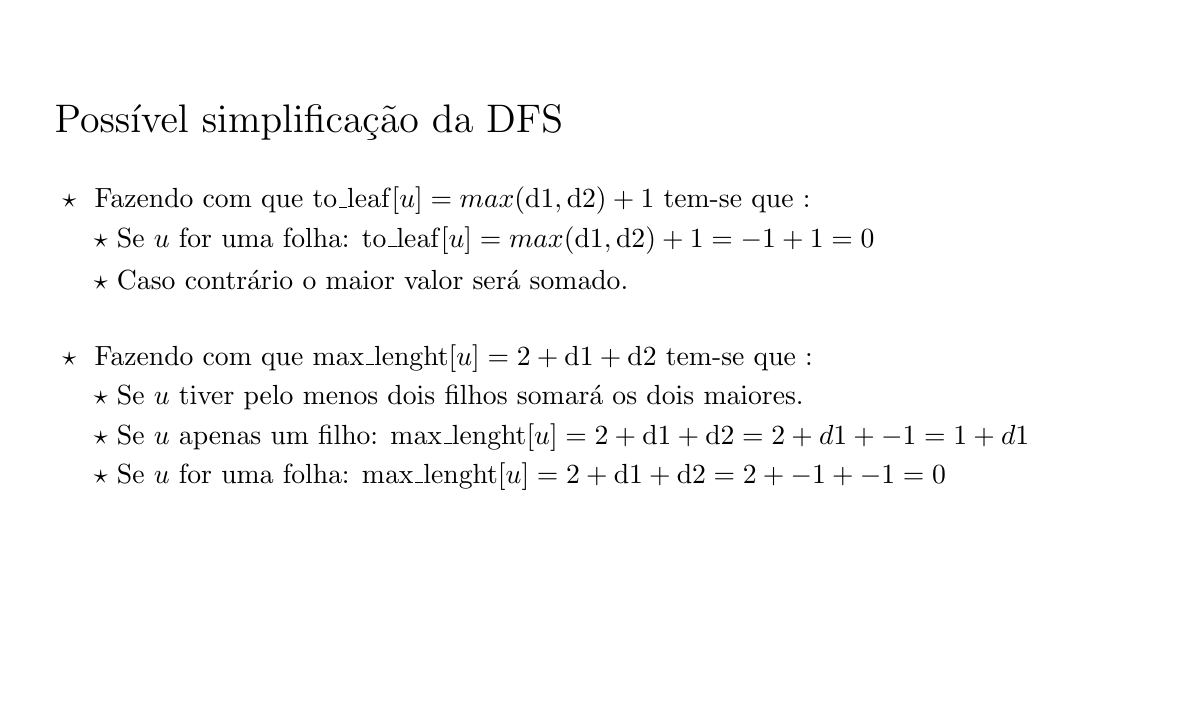
\begin{tikzpicture}
\node[draw,opacity=0] at (0, 0) {x};
\node[draw,opacity=0] at (14, 8) {x};
	\node[anchor=west] (title) at (0.0, 7.0) { \Large \bbbold{Possível simplificação da DFS} };

  \node[anchor=west] (a) at (0.1, 6.0) { $\star$ \bbtext{ Fazendo com que  $\displaystyle \mathrm{to\_leaf}[u] = max(\displaystyle \mathrm{d1}, \displaystyle \mathrm{d2}) + 1$ tem-se que :}  };
  \node[anchor=west] (a) at (0.5, 5.5) { $\star$ \bbtext{Se $u$ for uma folha:  $\displaystyle \mathrm{to\_leaf}[u] = max(\displaystyle \mathrm{d1}, \displaystyle \mathrm{d2}) + 1 = -1 + 1= 0$}  };
  \node[anchor=west] (a) at (0.5, 5.0) { $\star$ \bbtext{Caso contrário o maior valor será somado.}  };


  \node[anchor=west] (a) at (0.1, 4.0) { $\star$ \bbtext{ Fazendo com que  $\displaystyle \mathrm{max\_lenght}[u] = 2 + \displaystyle \mathrm{d1} + \displaystyle \mathrm{d2}$ tem-se que :}  };

  \node[anchor=west] (a) at (0.5, 3.5) { $\star$ \bbtext{Se $u$ tiver pelo menos dois filhos somará os dois maiores.}  };
  \node[anchor=west] (a) at (0.5, 3.0) { $\star$ \bbtext{Se $u$ apenas um filho: $\displaystyle \mathrm{max\_lenght}[u] = 2 + \displaystyle \mathrm{d1} + \displaystyle \mathrm{d2} = 2  + d1 + -1 = 1 +  d1$}  };
  \node[anchor=west] (a) at (0.5, 2.5) { $\star$ \bbtext{Se $u$ for uma folha: $\displaystyle \mathrm{max\_lenght}[u] = 2 + \displaystyle \mathrm{d1} + \displaystyle \mathrm{d2} = 2  + -1 + -1 = 0$}  };

\end{tikzpicture}
\end{frame}

\begin{frame}[plain,t]

  \inputsnippet{cpp}{10}{30}{codes/dp2.cpp}

\end{frame}

\begin{frame}[plain,t]
\begin{tikzpicture}
\node[draw,opacity=0] at (0, 0) {x};
\node[draw,opacity=0] at (14, 8) {x};

	\node[anchor=west] (title) at (0.0, 7.0) { \Large \bbbold{Uso de BFS para o cálculo do diâmetro} };

\end{tikzpicture}
\end{frame}
\begin{frame}[plain,t]
\begin{tikzpicture}
\node[draw,opacity=0] at (0, 0) {x};
\node[draw,opacity=0] at (14, 8) {x};

	\node[anchor=west] (title) at (0.0, 7.0) { \Large \bbbold{Uso de BFS para o cálculo do diâmetro} };


	\node[] (info) at (7.0, 6.0) { \bbtext{A BFS permite computar as distância, em arestas, de qualquer vértice a $u$} };

	\node[draw,thick,circle] (nodeA) at (1.0, 0.5) { \footnotesize $\textcolor{BBWhite}{a}$ };

	\node[fill=BBGreen,draw,thick,circle] (nodeU) at (3.0, 1.5) { \footnotesize $\textcolor{BBWhite}{u}$ };

	\node[draw,thick,circle] (nodeB) at (5.0, 2.5) { \footnotesize $\textcolor{BBWhite}{r}$ };

	\node[] (dots1) at (8.0, 2.5) { $\texttt{...}$ };

	\node[] (dots2) at (9.0, 3.5) { $\texttt{...}$ };

	\node[draw,thick,circle] (nodeC) at (11.0, 2.5) { \footnotesize $\textcolor{BBWhite}{c}$ };

	\node[draw,thick,circle] (nodeV) at (13.0, 0.5) { \footnotesize $\textcolor{BBWhite}{v}$ };

	\node[draw,thick,circle] (nodeP) at (1.0, 3.5) { \footnotesize $\textcolor{BBWhite}{p}$ };

	\node[draw,thick,circle] (nodeD) at (3.0, 4.5) { \footnotesize $\textcolor{BBWhite}{e}$ };

	\node[draw,thick,circle] (nodeE) at (5.0, 3.5) { \footnotesize $\textcolor{BBWhite}{e}$ };

	\node[draw,thick,circle] (nodeF) at (7.0, 3.5) { \footnotesize $\textcolor{BBWhite}{s}$ };

	\node[draw,thick,circle] (nodeG) at (11.0, 3.5) { \footnotesize $\textcolor{BBWhite}{e}$ };

	\node[draw,thick,circle] (nodeQ) at (13.0, 3.5) { \footnotesize $\textcolor{BBWhite}{q}$ };

	\draw[thick](nodeA) to (nodeU);

	\draw[thick](nodeB) to (nodeU);

	\draw[thick](nodeC) to (nodeV);

	\draw[thick](nodeP) to (nodeD);

	\draw[thick](nodeD) to (nodeE);

	\draw[thick](nodeE) to (nodeF);

	\draw[thick](nodeG) to (nodeQ);

	\draw[thick](nodeB) to (nodeF);

\end{tikzpicture}
\end{frame}
\begin{frame}[plain,t]
\begin{tikzpicture}
\node[draw,opacity=0] at (0, 0) {x};
\node[draw,opacity=0] at (14, 8) {x};

	\node[anchor=west] (title) at (0.0, 7.0) { \Large \bbbold{Uso de BFS para o cálculo do diâmetro} };


	\node[] (info) at (7.0, 6.0) { \bbtext{Seja $v$ o vértice mais distante de $u$ e $D$ o diâmetro da árvore $T$} };

	\node[draw,thick,circle] (nodeA) at (1.0, 0.5) { \footnotesize $\textcolor{BBWhite}{a}$ };

	\node[fill=BBGreen,draw,thick,circle] (nodeU) at (3.0, 1.5) { \footnotesize $\textcolor{BBWhite}{u}$ };

	\node[draw,thick,circle] (nodeB) at (5.0, 2.5) { \footnotesize $\textcolor{BBWhite}{r}$ };

	\node[] (dots1) at (8.0, 2.5) { $\texttt{...}$ };

	\node[] (dots2) at (9.0, 3.5) { $\texttt{...}$ };

	\node[draw,thick,circle] (nodeC) at (11.0, 2.5) { \footnotesize $\textcolor{BBWhite}{c}$ };

	\node[draw,thick,circle] (nodeV) at (13.0, 0.5) { \footnotesize $\textcolor{BBWhite}{v}$ };

	\node[draw,thick,circle] (nodeP) at (1.0, 3.5) { \footnotesize $\textcolor{BBWhite}{p}$ };

	\node[draw,thick,circle] (nodeD) at (3.0, 4.5) { \footnotesize $\textcolor{BBWhite}{e}$ };

	\node[draw,thick,circle] (nodeE) at (5.0, 3.5) { \footnotesize $\textcolor{BBWhite}{e}$ };

	\node[draw,thick,circle] (nodeF) at (7.0, 3.5) { \footnotesize $\textcolor{BBWhite}{s}$ };

	\node[draw,thick,circle] (nodeG) at (11.0, 3.5) { \footnotesize $\textcolor{BBWhite}{e}$ };

	\node[draw,thick,circle] (nodeQ) at (13.0, 3.5) { \footnotesize $\textcolor{BBWhite}{q}$ };

	\draw[thick](nodeA) to (nodeU);

	\draw[thick](nodeB) to (nodeU);

	\draw[thick](nodeC) to (nodeV);

	\draw[thick](nodeP) to (nodeD);

	\draw[thick](nodeD) to (nodeE);

	\draw[thick](nodeE) to (nodeF);

	\draw[thick](nodeG) to (nodeQ);

	\draw[thick](nodeB) to (nodeF);



\end{tikzpicture}
\end{frame}
\begin{frame}[plain,t]
\begin{tikzpicture}
\node[draw,opacity=0] at (0, 0) {x};
\node[draw,opacity=0] at (14, 8) {x};

	\node[anchor=west] (title) at (0.0, 7.0) { \Large \bbbold{Uso de BFS para o cálculo do diâmetro} };


	\node[] (info) at (7.0, 6.0) { \bbtext{Seja $v$ o vértice mais distante de $u$ e $D$ o diâmetro da árvore $T$} };

	\node[draw,thick,circle] (nodeA) at (1.0, 0.5) { \footnotesize $\textcolor{BBWhite}{a}$ };

	\node[fill=BBGreen,draw,thick,circle] (nodeU) at (3.0, 1.5) { \footnotesize $\textcolor{BBWhite}{u}$ };

	\node[draw,thick,circle] (nodeB) at (5.0, 2.5) { \footnotesize $\textcolor{BBWhite}{r}$ };

	\node[] (dots1) at (8.0, 2.5) { $\texttt{...}$ };

	\node[] (dots2) at (9.0, 3.5) { $\texttt{...}$ };

	\node[draw,thick,circle] (nodeC) at (11.0, 2.5) { \footnotesize $\textcolor{BBWhite}{c}$ };

	\node[draw,thick,circle,fill=BBCyan] (nodeV) at (13.0, 0.5) { \footnotesize $\textcolor{BBWhite}{v}$ };

	\node[draw,thick,circle] (nodeP) at (1.0, 3.5) { \footnotesize $\textcolor{BBWhite}{p}$ };

	\node[draw,thick,circle] (nodeD) at (3.0, 4.5) { \footnotesize $\textcolor{BBWhite}{e}$ };

	\node[draw,thick,circle] (nodeE) at (5.0, 3.5) { \footnotesize $\textcolor{BBWhite}{e}$ };

	\node[draw,thick,circle] (nodeF) at (7.0, 3.5) { \footnotesize $\textcolor{BBWhite}{s}$ };

	\node[draw,thick,circle] (nodeG) at (11.0, 3.5) { \footnotesize $\textcolor{BBWhite}{e}$ };

	\node[draw,thick,circle] (nodeQ) at (13.0, 3.5) { \footnotesize $\textcolor{BBWhite}{q}$ };

	\draw[thick](nodeA) to (nodeU);

	\draw[thick](nodeB) to (nodeU);

	\draw[thick](nodeC) to (nodeV);

	\draw[thick](nodeP) to (nodeD);

	\draw[thick](nodeD) to (nodeE);

	\draw[thick](nodeE) to (nodeF);

	\draw[thick](nodeG) to (nodeQ);

	\draw[thick](nodeB) to (nodeF);





\end{tikzpicture}
\end{frame}
\begin{frame}[plain,t]
\begin{tikzpicture}
\node[draw,opacity=0] at (0, 0) {x};
\node[draw,opacity=0] at (14, 8) {x};

	\node[anchor=west] (title) at (0.0, 7.0) { \Large \bbbold{Uso de BFS para o cálculo do diâmetro} };


	\node[] (info) at (7.0, 6.0) { \bbbold{Fato \#1:} \bbtext{Ao menos um nó do caminho de $u$ a $v$ faz parte de um} };

	\node[draw,thick,circle] (nodeA) at (1.0, 0.5) { \footnotesize $\textcolor{BBWhite}{a}$ };

	\node[fill=BBGreen,draw,thick,circle] (nodeU) at (3.0, 1.5) { \footnotesize $\textcolor{BBWhite}{u}$ };

	\node[draw,thick,circle] (nodeB) at (5.0, 2.5) { \footnotesize $\textcolor{BBWhite}{r}$ };

	\node[] (dots1) at (8.0, 2.5) { $\texttt{...}$ };

	\node[] (dots2) at (9.0, 3.5) { $\texttt{...}$ };

	\node[draw,thick,circle] (nodeC) at (11.0, 2.5) { \footnotesize $\textcolor{BBWhite}{c}$ };

	\node[draw,thick,circle,fill=BBCyan] (nodeV) at (13.0, 0.5) { \footnotesize $\textcolor{BBWhite}{v}$ };

	\node[draw,thick,circle] (nodeP) at (1.0, 3.5) { \footnotesize $\textcolor{BBWhite}{p}$ };

	\node[draw,thick,circle] (nodeD) at (3.0, 4.5) { \footnotesize $\textcolor{BBWhite}{e}$ };

	\node[draw,thick,circle] (nodeE) at (5.0, 3.5) { \footnotesize $\textcolor{BBWhite}{e}$ };

	\node[draw,thick,circle] (nodeF) at (7.0, 3.5) { \footnotesize $\textcolor{BBWhite}{s}$ };

	\node[draw,thick,circle] (nodeG) at (11.0, 3.5) { \footnotesize $\textcolor{BBWhite}{e}$ };

	\node[draw,thick,circle] (nodeQ) at (13.0, 3.5) { \footnotesize $\textcolor{BBWhite}{q}$ };

	\draw[thick](nodeA) to (nodeU);

	\draw[thick](nodeB) to (nodeU);

	\draw[thick](nodeC) to (nodeV);

	\draw[thick](nodeP) to (nodeD);

	\draw[thick](nodeD) to (nodeE);

	\draw[thick](nodeE) to (nodeF);

	\draw[thick](nodeG) to (nodeQ);

	\draw[thick](nodeB) to (nodeF);







	\node[] (info2) at (7.0, 5.5) { \bbtext{caminho cujo comprimento é $D$} };

\end{tikzpicture}
\end{frame}
\begin{frame}[plain,t]
\begin{tikzpicture}
\node[draw,opacity=0] at (0, 0) {x};
\node[draw,opacity=0] at (14, 8) {x};

	\node[anchor=west] (title) at (0.0, 7.0) { \Large \bbbold{Uso de BFS para o cálculo do diâmetro} };


	\node[] (info) at (7.0, 6.0) { \bbbold{Prova:} \bbtext{Suponha que nenhum vértice do caminho de $u$ a $v$ faça parte} };

	\node[draw,thick,circle] (nodeA) at (1.0, 0.5) { \footnotesize $\textcolor{BBWhite}{a}$ };

	\node[fill=BBGreen,draw,thick,circle] (nodeU) at (3.0, 1.5) { \footnotesize $\textcolor{BBWhite}{u}$ };

	\node[draw,thick,circle] (nodeB) at (5.0, 2.5) { \footnotesize $\textcolor{BBWhite}{r}$ };

	\node[] (dots1) at (8.0, 2.5) { $\texttt{...}$ };

	\node[] (dots2) at (9.0, 3.5) { $\texttt{...}$ };

	\node[draw,thick,circle] (nodeC) at (11.0, 2.5) { \footnotesize $\textcolor{BBWhite}{c}$ };

	\node[draw,thick,circle,fill=BBCyan] (nodeV) at (13.0, 0.5) { \footnotesize $\textcolor{BBWhite}{v}$ };

	\node[draw,thick,circle] (nodeP) at (1.0, 3.5) { \footnotesize $\textcolor{BBWhite}{p}$ };

	\node[draw,thick,circle] (nodeD) at (3.0, 4.5) { \footnotesize $\textcolor{BBWhite}{e}$ };

	\node[draw,thick,circle] (nodeE) at (5.0, 3.5) { \footnotesize $\textcolor{BBWhite}{e}$ };

	\node[draw,thick,circle] (nodeF) at (7.0, 3.5) { \footnotesize $\textcolor{BBWhite}{s}$ };

	\node[draw,thick,circle] (nodeG) at (11.0, 3.5) { \footnotesize $\textcolor{BBWhite}{e}$ };

	\node[draw,thick,circle] (nodeQ) at (13.0, 3.5) { \footnotesize $\textcolor{BBWhite}{q}$ };

	\draw[thick](nodeA) to (nodeU);

	\draw[thick](nodeB) to (nodeU);

	\draw[thick](nodeC) to (nodeV);

	\draw[thick](nodeP) to (nodeD);

	\draw[thick](nodeD) to (nodeE);

	\draw[thick](nodeE) to (nodeF);

	\draw[thick](nodeG) to (nodeQ);

	\draw[thick](nodeB) to (nodeF);







	\node[] (info2) at (7.0, 5.5) { \bbtext{de um caminho cujo comprimento é $D$} };



\end{tikzpicture}
\end{frame}
\begin{frame}[plain,t]
\begin{tikzpicture}
\node[draw,opacity=0] at (0, 0) {x};
\node[draw,opacity=0] at (14, 8) {x};

	\node[anchor=west] (title) at (0.0, 7.0) { \Large \bbbold{Uso de BFS para o cálculo do diâmetro} };


	\node[] (info) at (7.0, 6.0) { \bbtext{Assuma que $\dist(p, q) = D$} };

	\node[draw,thick,circle] (nodeA) at (1.0, 0.5) { \footnotesize $\textcolor{BBWhite}{a}$ };

	\node[fill=BBGreen,draw,thick,circle] (nodeU) at (3.0, 1.5) { \footnotesize $\textcolor{BBWhite}{u}$ };

	\node[draw,thick,circle] (nodeB) at (5.0, 2.5) { \footnotesize $\textcolor{BBWhite}{r}$ };

	\node[] (dots1) at (8.0, 2.5) { $\texttt{...}$ };

	\node[] (dots2) at (9.0, 3.5) { $\texttt{...}$ };

	\node[draw,thick,circle] (nodeC) at (11.0, 2.5) { \footnotesize $\textcolor{BBWhite}{c}$ };

	\node[draw,thick,circle,fill=BBCyan] (nodeV) at (13.0, 0.5) { \footnotesize $\textcolor{BBWhite}{v}$ };

	\node[draw,thick,circle,fill=BBOrange] (nodeP) at (1.0, 3.5) { \footnotesize $\textcolor{BBWhite}{p}$ };

	\node[draw,thick,circle] (nodeD) at (3.0, 4.5) { \footnotesize $\textcolor{BBWhite}{e}$ };

	\node[draw,thick,circle] (nodeE) at (5.0, 3.5) { \footnotesize $\textcolor{BBWhite}{e}$ };

	\node[draw,thick,circle] (nodeF) at (7.0, 3.5) { \footnotesize $\textcolor{BBWhite}{s}$ };

	\node[draw,thick,circle] (nodeG) at (11.0, 3.5) { \footnotesize $\textcolor{BBWhite}{e}$ };

	\node[draw,thick,circle,fill=BBOrange] (nodeQ) at (13.0, 3.5) { \footnotesize $\textcolor{BBWhite}{q}$ };

	\draw[thick](nodeA) to (nodeU);

	\draw[thick](nodeB) to (nodeU);

	\draw[thick](nodeC) to (nodeV);

	\draw[thick,dashed](nodeP) to (nodeD);

	\draw[thick,dashed](nodeD) to (nodeE);

	\draw[thick,dashed](nodeE) to (nodeF);

	\draw[thick,dashed](nodeG) to (nodeQ);

	\draw[thick](nodeB) to (nodeF);














\end{tikzpicture}
\end{frame}
\begin{frame}[plain,t]
\begin{tikzpicture}
\node[draw,opacity=0] at (0, 0) {x};
\node[draw,opacity=0] at (14, 8) {x};

	\node[anchor=west] (title) at (0.0, 7.0) { \Large \bbbold{Uso de BFS para o cálculo do diâmetro} };


	\node[] (info) at (7.0, 6.0) { \bbtext{Sendo $T$ conectada, existe ao menos um caminho de um vértice $r$} };

	\node[draw,thick,circle] (nodeA) at (1.0, 0.5) { \footnotesize $\textcolor{BBWhite}{a}$ };

	\node[fill=BBGreen,draw,thick,circle] (nodeU) at (3.0, 1.5) { \footnotesize $\textcolor{BBWhite}{u}$ };

	\node[draw,thick,circle] (nodeB) at (5.0, 2.5) { \footnotesize $\textcolor{BBWhite}{r}$ };

	\node[] (dots1) at (8.0, 2.5) { $\texttt{...}$ };

	\node[] (dots2) at (9.0, 3.5) { $\texttt{...}$ };

	\node[draw,thick,circle] (nodeC) at (11.0, 2.5) { \footnotesize $\textcolor{BBWhite}{c}$ };

	\node[draw,thick,circle,fill=BBCyan] (nodeV) at (13.0, 0.5) { \footnotesize $\textcolor{BBWhite}{v}$ };

	\node[draw,thick,circle,fill=BBOrange] (nodeP) at (1.0, 3.5) { \footnotesize $\textcolor{BBWhite}{p}$ };

	\node[draw,thick,circle] (nodeD) at (3.0, 4.5) { \footnotesize $\textcolor{BBWhite}{e}$ };

	\node[draw,thick,circle] (nodeE) at (5.0, 3.5) { \footnotesize $\textcolor{BBWhite}{e}$ };

	\node[draw,thick,circle] (nodeF) at (7.0, 3.5) { \footnotesize $\textcolor{BBWhite}{s}$ };

	\node[draw,thick,circle] (nodeG) at (11.0, 3.5) { \footnotesize $\textcolor{BBWhite}{e}$ };

	\node[draw,thick,circle,fill=BBOrange] (nodeQ) at (13.0, 3.5) { \footnotesize $\textcolor{BBWhite}{q}$ };

	\draw[thick](nodeA) to (nodeU);

	\draw[thick](nodeB) to (nodeU);

	\draw[thick](nodeC) to (nodeV);

	\draw[thick,dashed](nodeP) to (nodeD);

	\draw[thick,dashed](nodeD) to (nodeE);

	\draw[thick,dashed](nodeE) to (nodeF);

	\draw[thick,dashed](nodeG) to (nodeQ);

	\draw[thick](nodeB) to (nodeF);







	\node[] (info2) at (7.0, 5.5) { \bbtext{no caminho de $u$ a $v$ para um vértice $s$ no caminho de $p$ a $q$} };









\end{tikzpicture}
\end{frame}
\begin{frame}[plain,t]
\begin{tikzpicture}
\node[draw,opacity=0] at (0, 0) {x};
\node[draw,opacity=0] at (14, 8) {x};

	\node[anchor=west] (title) at (0.0, 7.0) { \Large \bbbold{Uso de BFS para o cálculo do diâmetro} };


	\node[] (info) at (7.0, 6.0) { \bbtext{Sendo $T$ conectada, existe ao menos um caminho de um vértice $r$} };

	\node[draw,thick,circle] (nodeA) at (1.0, 0.5) { \footnotesize $\textcolor{BBWhite}{a}$ };

	\node[fill=BBGreen,draw,thick,circle] (nodeU) at (3.0, 1.5) { \footnotesize $\textcolor{BBWhite}{u}$ };

	\node[draw,thick,circle,fill=BBGray] (nodeB) at (5.0, 2.5) { \footnotesize $\textcolor{BBWhite}{r}$ };

	\node[] (dots1) at (8.0, 2.5) { $\texttt{...}$ };

	\node[] (dots2) at (9.0, 3.5) { $\texttt{...}$ };

	\node[draw,thick,circle] (nodeC) at (11.0, 2.5) { \footnotesize $\textcolor{BBWhite}{c}$ };

	\node[draw,thick,circle,fill=BBCyan] (nodeV) at (13.0, 0.5) { \footnotesize $\textcolor{BBWhite}{v}$ };

	\node[draw,thick,circle,fill=BBOrange] (nodeP) at (1.0, 3.5) { \footnotesize $\textcolor{BBWhite}{p}$ };

	\node[draw,thick,circle] (nodeD) at (3.0, 4.5) { \footnotesize $\textcolor{BBWhite}{e}$ };

	\node[draw,thick,circle] (nodeE) at (5.0, 3.5) { \footnotesize $\textcolor{BBWhite}{e}$ };

	\node[draw,thick,circle,fill=BBGray] (nodeF) at (7.0, 3.5) { \footnotesize $\textcolor{BBWhite}{s}$ };

	\node[draw,thick,circle] (nodeG) at (11.0, 3.5) { \footnotesize $\textcolor{BBWhite}{e}$ };

	\node[draw,thick,circle,fill=BBOrange] (nodeQ) at (13.0, 3.5) { \footnotesize $\textcolor{BBWhite}{q}$ };

	\draw[thick](nodeA) to (nodeU);

	\draw[thick](nodeB) to (nodeU);

	\draw[thick](nodeC) to (nodeV);

	\draw[thick,dashed](nodeP) to (nodeD);

	\draw[thick,dashed](nodeD) to (nodeE);

	\draw[thick,dashed](nodeE) to (nodeF);

	\draw[thick,dashed](nodeG) to (nodeQ);

	\draw[thick,-latex,very thick](nodeB) to (nodeF);







	\node[] (info2) at (7.0, 5.5) { \bbtext{no caminho de $u$ a $v$ para um vértice $s$ no caminho de $p$ a $q$} };











\end{tikzpicture}
\end{frame}
\begin{frame}[plain,t]
\begin{tikzpicture}
\node[draw,opacity=0] at (0, 0) {x};
\node[draw,opacity=0] at (14, 8) {x};

	\node[anchor=west] (title) at (0.0, 7.0) { \Large \bbbold{Uso de BFS para o cálculo do diâmetro} };


	\node[] (info) at (7.0, 6.0) { \bbtext{Como $v$ é vértice mais distante de $u$, vale que} };

	\node[draw,thick,circle] (nodeA) at (1.0, 0.5) { \footnotesize $\textcolor{BBWhite}{a}$ };

	\node[fill=BBGreen,draw,thick,circle] (nodeU) at (3.0, 1.5) { \footnotesize $\textcolor{BBWhite}{u}$ };

	\node[draw,thick,circle,fill=BBGray] (nodeB) at (5.0, 2.5) { \footnotesize $\textcolor{BBWhite}{r}$ };

	\node[] (dots1) at (8.0, 2.5) { $\texttt{...}$ };

	\node[] (dots2) at (9.0, 3.5) { $\texttt{...}$ };

	\node[draw,thick,circle] (nodeC) at (11.0, 2.5) { \footnotesize $\textcolor{BBWhite}{c}$ };

	\node[draw,thick,circle,fill=BBCyan] (nodeV) at (13.0, 0.5) { \footnotesize $\textcolor{BBWhite}{v}$ };

	\node[draw,thick,circle,fill=BBOrange] (nodeP) at (1.0, 3.5) { \footnotesize $\textcolor{BBWhite}{p}$ };

	\node[draw,thick,circle] (nodeD) at (3.0, 4.5) { \footnotesize $\textcolor{BBWhite}{e}$ };

	\node[draw,thick,circle] (nodeE) at (5.0, 3.5) { \footnotesize $\textcolor{BBWhite}{e}$ };

	\node[draw,thick,circle,fill=BBGray] (nodeF) at (7.0, 3.5) { \footnotesize $\textcolor{BBWhite}{s}$ };

	\node[draw,thick,circle] (nodeG) at (11.0, 3.5) { \footnotesize $\textcolor{BBWhite}{e}$ };

	\node[draw,thick,circle,fill=BBOrange] (nodeQ) at (13.0, 3.5) { \footnotesize $\textcolor{BBWhite}{q}$ };

	\draw[thick](nodeA) to (nodeU);

	\draw[thick](nodeB) to (nodeU);

	\draw[thick](nodeC) to (nodeV);

	\draw[thick,dashed](nodeP) to (nodeD);

	\draw[thick,dashed](nodeD) to (nodeE);

	\draw[thick,dashed](nodeE) to (nodeF);

	\draw[thick,dashed](nodeG) to (nodeQ);

	\draw[thick,-latex,very thick](nodeB) to (nodeF);







	\node[] (info2) at (7.0, 5.25) { $\displaystyle \dist(u, r) + \dist(r, s) + \dist(s, p) \leq \dist(u, v)$ };













\end{tikzpicture}
\end{frame}
\begin{frame}[plain,t]
\begin{tikzpicture}
\node[draw,opacity=0] at (0, 0) {x};
\node[draw,opacity=0] at (14, 8) {x};

	\node[anchor=west] (title) at (0.0, 7.0) { \Large \bbbold{Uso de BFS para o cálculo do diâmetro} };


	\node[] (info) at (7.0, 6.0) { \bbtext{Como $v$ é vértice mais distante de $u$, vale que} };

	\node[draw,thick,circle] (nodeA) at (1.0, 0.5) { \footnotesize $\textcolor{BBWhite}{a}$ };

	\node[fill=BBGreen,draw,thick,circle] (nodeU) at (3.0, 1.5) { \footnotesize $\textcolor{BBWhite}{u}$ };

	\node[draw,thick,circle,fill=BBGray] (nodeB) at (5.0, 2.5) { \footnotesize $\textcolor{BBWhite}{r}$ };

	\node[] (dots1) at (8.0, 2.5) { $\texttt{...}$ };

	\node[] (dots2) at (9.0, 3.5) { $\texttt{...}$ };

	\node[draw,thick,circle] (nodeC) at (11.0, 2.5) { \footnotesize $\textcolor{BBWhite}{c}$ };

	\node[draw,thick,circle,fill=BBCyan] (nodeV) at (13.0, 0.5) { \footnotesize $\textcolor{BBWhite}{v}$ };

	\node[draw,thick,circle,fill=BBOrange] (nodeP) at (1.0, 3.5) { \footnotesize $\textcolor{BBWhite}{p}$ };

	\node[draw,thick,circle] (nodeD) at (3.0, 4.5) { \footnotesize $\textcolor{BBWhite}{e}$ };

	\node[draw,thick,circle] (nodeE) at (5.0, 3.5) { \footnotesize $\textcolor{BBWhite}{e}$ };

	\node[draw,thick,circle,fill=BBGray] (nodeF) at (7.0, 3.5) { \footnotesize $\textcolor{BBWhite}{s}$ };

	\node[draw,thick,circle] (nodeG) at (11.0, 3.5) { \footnotesize $\textcolor{BBWhite}{e}$ };

	\node[draw,thick,circle,fill=BBOrange] (nodeQ) at (13.0, 3.5) { \footnotesize $\textcolor{BBWhite}{q}$ };

	\draw[thick](nodeA) to (nodeU);

	\draw[thick](nodeB) to (nodeU);

	\draw[thick](nodeC) to (nodeV);

	\draw[thick,dashed](nodeP) to (nodeD);

	\draw[thick,dashed](nodeD) to (nodeE);

	\draw[thick,dashed](nodeE) to (nodeF);

	\draw[thick,dashed](nodeG) to (nodeQ);

	\draw[thick,-latex,very thick](nodeB) to (nodeF);







	\node[] (info2) at (7.0, 5.25) { $\displaystyle \dist(u, r) + \dist(r, s) + \dist(s, p) \leq \dist(u, v)$ };














	\draw[color=BBViolet,-latex](nodeU) to [bend left] (nodeB);

	\draw[color=BBViolet,-latex](nodeB) to [bend right] (nodeF);

	\draw[color=BBViolet,-latex](nodeF) to [bend right] (nodeE);

	\draw[color=BBViolet,-latex](nodeE) to [bend left] (nodeD);

	\draw[color=BBViolet,-latex](nodeD) to [bend right] (nodeP);

\end{tikzpicture}
\end{frame}
\begin{frame}[plain,t]
\begin{tikzpicture}
\node[draw,opacity=0] at (0, 0) {x};
\node[draw,opacity=0] at (14, 8) {x};

	\node[anchor=west] (title) at (0.0, 7.0) { \Large \bbbold{Uso de BFS para o cálculo do diâmetro} };


	\node[] (info) at (7.0, 6.0) { \bbtext{e também que} };

	\node[draw,thick,circle] (nodeA) at (1.0, 0.5) { \footnotesize $\textcolor{BBWhite}{a}$ };

	\node[fill=BBGreen,draw,thick,circle] (nodeU) at (3.0, 1.5) { \footnotesize $\textcolor{BBWhite}{u}$ };

	\node[draw,thick,circle,fill=BBGray] (nodeB) at (5.0, 2.5) { \footnotesize $\textcolor{BBWhite}{r}$ };

	\node[] (dots1) at (8.0, 2.5) { $\texttt{...}$ };

	\node[] (dots2) at (9.0, 3.5) { $\texttt{...}$ };

	\node[draw,thick,circle] (nodeC) at (11.0, 2.5) { \footnotesize $\textcolor{BBWhite}{c}$ };

	\node[draw,thick,circle,fill=BBCyan] (nodeV) at (13.0, 0.5) { \footnotesize $\textcolor{BBWhite}{v}$ };

	\node[draw,thick,circle,fill=BBOrange] (nodeP) at (1.0, 3.5) { \footnotesize $\textcolor{BBWhite}{p}$ };

	\node[draw,thick,circle] (nodeD) at (3.0, 4.5) { \footnotesize $\textcolor{BBWhite}{e}$ };

	\node[draw,thick,circle] (nodeE) at (5.0, 3.5) { \footnotesize $\textcolor{BBWhite}{e}$ };

	\node[draw,thick,circle,fill=BBGray] (nodeF) at (7.0, 3.5) { \footnotesize $\textcolor{BBWhite}{s}$ };

	\node[draw,thick,circle] (nodeG) at (11.0, 3.5) { \footnotesize $\textcolor{BBWhite}{e}$ };

	\node[draw,thick,circle,fill=BBOrange] (nodeQ) at (13.0, 3.5) { \footnotesize $\textcolor{BBWhite}{q}$ };

	\draw[thick](nodeA) to (nodeU);

	\draw[thick](nodeB) to (nodeU);

	\draw[thick](nodeC) to (nodeV);

	\draw[thick,dashed](nodeP) to (nodeD);

	\draw[thick,dashed](nodeD) to (nodeE);

	\draw[thick,dashed](nodeE) to (nodeF);

	\draw[thick,dashed](nodeG) to (nodeQ);

	\draw[thick,-latex,very thick](nodeB) to (nodeF);







	\node[] (info2) at (7.0, 5.25) { $\displaystyle \dist(v, r) + \dist(r, s) + \dist(s, q) \leq \dist(u, v)$ };





















\end{tikzpicture}
\end{frame}
\begin{frame}[plain,t]
\begin{tikzpicture}
\node[draw,opacity=0] at (0, 0) {x};
\node[draw,opacity=0] at (14, 8) {x};

	\node[anchor=west] (title) at (0.0, 7.0) { \Large \bbbold{Uso de BFS para o cálculo do diâmetro} };


	\node[] (info) at (7.0, 6.0) { \bbtext{e também que} };

	\node[draw,thick,circle] (nodeA) at (1.0, 0.5) { \footnotesize $\textcolor{BBWhite}{a}$ };

	\node[fill=BBGreen,draw,thick,circle] (nodeU) at (3.0, 1.5) { \footnotesize $\textcolor{BBWhite}{u}$ };

	\node[draw,thick,circle,fill=BBGray] (nodeB) at (5.0, 2.5) { \footnotesize $\textcolor{BBWhite}{r}$ };

	\node[] (dots1) at (8.0, 2.5) { $\texttt{...}$ };

	\node[] (dots2) at (9.0, 3.5) { $\texttt{...}$ };

	\node[draw,thick,circle] (nodeC) at (11.0, 2.5) { \footnotesize $\textcolor{BBWhite}{c}$ };

	\node[draw,thick,circle,fill=BBCyan] (nodeV) at (13.0, 0.5) { \footnotesize $\textcolor{BBWhite}{v}$ };

	\node[draw,thick,circle,fill=BBOrange] (nodeP) at (1.0, 3.5) { \footnotesize $\textcolor{BBWhite}{p}$ };

	\node[draw,thick,circle] (nodeD) at (3.0, 4.5) { \footnotesize $\textcolor{BBWhite}{e}$ };

	\node[draw,thick,circle] (nodeE) at (5.0, 3.5) { \footnotesize $\textcolor{BBWhite}{e}$ };

	\node[draw,thick,circle,fill=BBGray] (nodeF) at (7.0, 3.5) { \footnotesize $\textcolor{BBWhite}{s}$ };

	\node[draw,thick,circle] (nodeG) at (11.0, 3.5) { \footnotesize $\textcolor{BBWhite}{e}$ };

	\node[draw,thick,circle,fill=BBOrange] (nodeQ) at (13.0, 3.5) { \footnotesize $\textcolor{BBWhite}{q}$ };

	\draw[thick](nodeA) to (nodeU);

	\draw[thick](nodeB) to (nodeU);

	\draw[thick](nodeC) to (nodeV);

	\draw[thick,dashed](nodeP) to (nodeD);

	\draw[thick,dashed](nodeD) to (nodeE);

	\draw[thick,dashed](nodeE) to (nodeF);

	\draw[thick,dashed](nodeG) to (nodeQ);

	\draw[thick,-latex,very thick](nodeB) to (nodeF);







	\node[] (info2) at (7.0, 5.25) { $\displaystyle \dist(v, r) + \dist(r, s) + \dist(s, q) \leq \dist(u, v)$ };















	\draw[color=BBViolet,-latex](nodeB) to [bend right] (nodeF);







	\draw[color=BBViolet,-latex](nodeV) to [bend right] (nodeC);

	\draw[color=BBViolet,-latex](nodeC) to [bend left] (nodeB);


	\draw[color=BBViolet,-latex](nodeF) to [bend left] (nodeG);

	\draw[color=BBViolet,-latex](nodeG) to [bend left] (nodeQ);

\end{tikzpicture}
\end{frame}
\begin{frame}[plain,t]
\begin{tikzpicture}
\node[draw,opacity=0] at (0, 0) {x};
\node[draw,opacity=0] at (14, 8) {x};

	\node[anchor=west] (title) at (0.0, 7.0) { \Large \bbbold{Uso de BFS para o cálculo do diâmetro} };


	\node[] (info) at (7.0, 6.0) { \bbtext{Somando ambas desigualdades, temos que} };

	\node[draw,thick,circle] (nodeA) at (1.0, 0.5) { \footnotesize $\textcolor{BBWhite}{a}$ };

	\node[fill=BBGreen,draw,thick,circle] (nodeU) at (3.0, 1.5) { \footnotesize $\textcolor{BBWhite}{u}$ };

	\node[draw,thick,circle,fill=BBGray] (nodeB) at (5.0, 2.5) { \footnotesize $\textcolor{BBWhite}{r}$ };

	\node[] (dots1) at (8.0, 2.5) { $\texttt{...}$ };

	\node[] (dots2) at (9.0, 3.5) { $\texttt{...}$ };

	\node[draw,thick,circle] (nodeC) at (11.0, 2.5) { \footnotesize $\textcolor{BBWhite}{c}$ };

	\node[draw,thick,circle,fill=BBCyan] (nodeV) at (13.0, 0.5) { \footnotesize $\textcolor{BBWhite}{v}$ };

	\node[draw,thick,circle,fill=BBOrange] (nodeP) at (1.0, 3.5) { \footnotesize $\textcolor{BBWhite}{p}$ };

	\node[draw,thick,circle] (nodeD) at (3.0, 4.5) { \footnotesize $\textcolor{BBWhite}{e}$ };

	\node[draw,thick,circle] (nodeE) at (5.0, 3.5) { \footnotesize $\textcolor{BBWhite}{e}$ };

	\node[draw,thick,circle,fill=BBGray] (nodeF) at (7.0, 3.5) { \footnotesize $\textcolor{BBWhite}{s}$ };

	\node[draw,thick,circle] (nodeG) at (11.0, 3.5) { \footnotesize $\textcolor{BBWhite}{e}$ };

	\node[draw,thick,circle,fill=BBOrange] (nodeQ) at (13.0, 3.5) { \footnotesize $\textcolor{BBWhite}{q}$ };

	\draw[thick](nodeA) to (nodeU);

	\draw[thick](nodeB) to (nodeU);

	\draw[thick](nodeC) to (nodeV);

	\draw[thick,dashed](nodeP) to (nodeD);

	\draw[thick,dashed](nodeD) to (nodeE);

	\draw[thick,dashed](nodeE) to (nodeF);

	\draw[thick,dashed](nodeG) to (nodeQ);

	\draw[thick,-latex,very thick](nodeB) to (nodeF);







	\node[] (info2) at (7.0, 5.25) { $\displaystyle D + 2\times \dist(r, s) \leq \dist(u, v)$ };





























\end{tikzpicture}
\end{frame}
\begin{frame}[plain,t]
\begin{tikzpicture}
\node[draw,opacity=0] at (0, 0) {x};
\node[draw,opacity=0] at (14, 8) {x};

	\node[anchor=west] (title) at (0.0, 7.0) { \Large \bbbold{Uso de BFS para o cálculo do diâmetro} };


	\node[] (info) at (7.0, 6.0) { \bbtext{Como $\dist(r, s) > 0$, teríamos $\dist(u, v) > D$, uma contradição!} };

	\node[draw,thick,circle] (nodeA) at (1.0, 0.5) { \footnotesize $\textcolor{BBWhite}{a}$ };

	\node[fill=BBGreen,draw,thick,circle] (nodeU) at (3.0, 1.5) { \footnotesize $\textcolor{BBWhite}{u}$ };

	\node[draw,thick,circle,fill=BBGray] (nodeB) at (5.0, 2.5) { \footnotesize $\textcolor{BBWhite}{r}$ };

	\node[] (dots1) at (8.0, 2.5) { $\texttt{...}$ };

	\node[] (dots2) at (9.0, 3.5) { $\texttt{...}$ };

	\node[draw,thick,circle] (nodeC) at (11.0, 2.5) { \footnotesize $\textcolor{BBWhite}{c}$ };

	\node[draw,thick,circle,fill=BBCyan] (nodeV) at (13.0, 0.5) { \footnotesize $\textcolor{BBWhite}{v}$ };

	\node[draw,thick,circle,fill=BBOrange] (nodeP) at (1.0, 3.5) { \footnotesize $\textcolor{BBWhite}{p}$ };

	\node[draw,thick,circle] (nodeD) at (3.0, 4.5) { \footnotesize $\textcolor{BBWhite}{e}$ };

	\node[draw,thick,circle] (nodeE) at (5.0, 3.5) { \footnotesize $\textcolor{BBWhite}{e}$ };

	\node[draw,thick,circle,fill=BBGray] (nodeF) at (7.0, 3.5) { \footnotesize $\textcolor{BBWhite}{s}$ };

	\node[draw,thick,circle] (nodeG) at (11.0, 3.5) { \footnotesize $\textcolor{BBWhite}{e}$ };

	\node[draw,thick,circle,fill=BBOrange] (nodeQ) at (13.0, 3.5) { \footnotesize $\textcolor{BBWhite}{q}$ };

	\draw[thick](nodeA) to (nodeU);

	\draw[thick](nodeB) to (nodeU);

	\draw[thick](nodeC) to (nodeV);

	\draw[thick,dashed](nodeP) to (nodeD);

	\draw[thick,dashed](nodeD) to (nodeE);

	\draw[thick,dashed](nodeE) to (nodeF);

	\draw[thick,dashed](nodeG) to (nodeQ);

	\draw[thick,-latex,very thick](nodeB) to (nodeF);






































\end{tikzpicture}
\end{frame}
\begin{frame}[plain,t]
\begin{tikzpicture}
\node[draw,opacity=0] at (0, 0) {x};
\node[draw,opacity=0] at (14, 8) {x};

	\node[anchor=west] (title) at (0.0, 7.0) { \Large \bbbold{Uso de BFS para o cálculo do diâmetro} };


	\node[] (info) at (7.0, 6.0) { \bbbold{Fato \#2:} \bbtext{$v$ é um dos extremos de um caminho cujo tamanho é $D$} };

	\node[draw,thick,circle] (nodeA) at (1.0, 0.5) { \footnotesize $\textcolor{BBWhite}{a}$ };

	\node[fill=BBGreen,draw,thick,circle] (nodeU) at (3.0, 1.5) { \footnotesize $\textcolor{BBWhite}{u}$ };

	\node[draw,thick,circle,fill=BBGray] (nodeB) at (5.0, 2.5) { \footnotesize $\textcolor{BBWhite}{r}$ };

	\node[] (dots1) at (8.0, 2.5) { $\texttt{...}$ };

	\node[] (dots2) at (9.0, 3.5) { $\texttt{...}$ };

	\node[draw,thick,circle] (nodeC) at (11.0, 2.5) { \footnotesize $\textcolor{BBWhite}{c}$ };

	\node[draw,thick,circle,fill=BBCyan] (nodeV) at (13.0, 0.5) { \footnotesize $\textcolor{BBWhite}{v}$ };

	\node[draw,thick,circle,fill=BBOrange] (nodeP) at (1.0, 3.5) { \footnotesize $\textcolor{BBWhite}{p}$ };

	\node[draw,thick,circle] (nodeD) at (3.0, 4.5) { \footnotesize $\textcolor{BBWhite}{e}$ };

	\node[draw,thick,circle] (nodeE) at (5.0, 3.5) { \footnotesize $\textcolor{BBWhite}{e}$ };

	\node[draw,thick,circle,fill=BBGray] (nodeF) at (7.0, 3.5) { \footnotesize $\textcolor{BBWhite}{s}$ };

	\node[draw,thick,circle] (nodeG) at (11.0, 3.5) { \footnotesize $\textcolor{BBWhite}{e}$ };

	\node[draw,thick,circle,fill=BBOrange] (nodeQ) at (13.0, 3.5) { \footnotesize $\textcolor{BBWhite}{q}$ };

	\draw[thick](nodeA) to (nodeU);

	\draw[thick](nodeB) to (nodeU);

	\draw[thick](nodeC) to (nodeV);

	\draw[thick,dashed](nodeP) to (nodeD);

	\draw[thick,dashed](nodeD) to (nodeE);

	\draw[thick,dashed](nodeE) to (nodeF);

	\draw[thick,dashed](nodeG) to (nodeQ);










































	\draw[thick](nodeB) to (nodeF);

\end{tikzpicture}
\end{frame}
\begin{frame}[plain,t]
\begin{tikzpicture}
\node[draw,opacity=0] at (0, 0) {x};
\node[draw,opacity=0] at (14, 8) {x};

	\node[anchor=west] (title) at (0.0, 7.0) { \Large \bbbold{Uso de BFS para o cálculo do diâmetro} };


	\node[] (info) at (7.0, 6.0) { \bbbold{Prova:} \bbtext{Seja $s$ um nó do caminho de $u$ a $v$ pelo qual passa o} };

	\node[draw,thick,circle] (nodeA) at (1.0, 0.5) { \footnotesize $\textcolor{BBWhite}{a}$ };

	\node[fill=BBGreen,draw,thick,circle] (nodeU) at (3.0, 1.5) { \footnotesize $\textcolor{BBWhite}{u}$ };

	\node[draw,thick,circle,fill=BBGray] (nodeB) at (5.0, 2.5) { \footnotesize $\textcolor{BBWhite}{r}$ };

	\node[] (dots1) at (8.0, 2.5) { $\texttt{...}$ };

	\node[] (dots2) at (9.0, 3.5) { $\texttt{...}$ };

	\node[draw,thick,circle] (nodeC) at (11.0, 2.5) { \footnotesize $\textcolor{BBWhite}{c}$ };

	\node[draw,thick,circle,fill=BBCyan] (nodeV) at (13.0, 0.5) { \footnotesize $\textcolor{BBWhite}{v}$ };

	\node[draw,thick,circle,fill=BBOrange] (nodeP) at (1.0, 3.5) { \footnotesize $\textcolor{BBWhite}{p}$ };

	\node[draw,thick,circle] (nodeD) at (3.0, 4.5) { \footnotesize $\textcolor{BBWhite}{e}$ };

	\node[draw,thick,circle] (nodeE) at (5.0, 3.5) { \footnotesize $\textcolor{BBWhite}{e}$ };

	\node[draw,thick,circle,fill=BBGray] (nodeF) at (7.0, 3.5) { \footnotesize $\textcolor{BBWhite}{s}$ };

	\node[draw,thick,circle] (nodeG) at (11.0, 3.5) { \footnotesize $\textcolor{BBWhite}{e}$ };

	\node[draw,thick,circle,fill=BBOrange] (nodeQ) at (13.0, 3.5) { \footnotesize $\textcolor{BBWhite}{q}$ };

	\draw[thick](nodeA) to (nodeU);

	\draw[thick](nodeB) to (nodeU);

	\draw[thick](nodeC) to (nodeV);

	\draw[thick,dashed](nodeP) to (nodeD);

	\draw[thick,dashed](nodeD) to (nodeE);

	\draw[thick,dashed](nodeE) to (nodeF);

	\draw[thick,dashed](nodeG) to (nodeQ);








	\node[] (info2) at (7.0, 5.5) { \bbtext{caminho de $p$ a $q$ cujo tamanho é $D$} };


































	\draw[thick](nodeB) to (nodeF);




\end{tikzpicture}
\end{frame}
\begin{frame}[plain,t]
\begin{tikzpicture}
\node[draw,opacity=0] at (0, 0) {x};
\node[draw,opacity=0] at (14, 8) {x};

	\node[anchor=west] (title) at (0.0, 7.0) { \Large \bbbold{Uso de BFS para o cálculo do diâmetro} };


	\node[] (info) at (7.0, 6.0) { \bbtext{Se $v$ não é extremo de um caminho cujo tamanho é $D$, então} };

	\node[draw,thick,circle] (nodeA) at (1.0, 0.5) { \footnotesize $\textcolor{BBWhite}{a}$ };

	\node[fill=BBGreen,draw,thick,circle] (nodeU) at (3.0, 1.5) { \footnotesize $\textcolor{BBWhite}{u}$ };

	\node[draw,thick,circle,fill=BBGray] (nodeB) at (5.0, 2.5) { \footnotesize $\textcolor{BBWhite}{r}$ };

	\node[] (dots1) at (8.0, 2.5) { $\texttt{...}$ };

	\node[] (dots2) at (9.0, 3.5) { $\texttt{...}$ };

	\node[draw,thick,circle] (nodeC) at (11.0, 2.5) { \footnotesize $\textcolor{BBWhite}{c}$ };

	\node[draw,thick,circle,fill=BBCyan] (nodeV) at (13.0, 0.5) { \footnotesize $\textcolor{BBWhite}{v}$ };

	\node[draw,thick,circle,fill=BBOrange] (nodeP) at (1.0, 3.5) { \footnotesize $\textcolor{BBWhite}{p}$ };

	\node[draw,thick,circle] (nodeD) at (3.0, 4.5) { \footnotesize $\textcolor{BBWhite}{e}$ };

	\node[draw,thick,circle] (nodeE) at (5.0, 3.5) { \footnotesize $\textcolor{BBWhite}{e}$ };

	\node[draw,thick,circle,fill=BBGray] (nodeF) at (7.0, 3.5) { \footnotesize $\textcolor{BBWhite}{s}$ };

	\node[draw,thick,circle] (nodeG) at (11.0, 3.5) { \footnotesize $\textcolor{BBWhite}{e}$ };

	\node[draw,thick,circle,fill=BBOrange] (nodeQ) at (13.0, 3.5) { \footnotesize $\textcolor{BBWhite}{q}$ };

	\draw[thick](nodeA) to (nodeU);

	\draw[thick](nodeB) to (nodeU);

	\draw[thick](nodeC) to (nodeV);

	\draw[thick,dashed](nodeP) to (nodeD);

	\draw[thick,dashed](nodeD) to (nodeE);

	\draw[thick,dashed](nodeE) to (nodeF);

	\draw[thick,dashed](nodeG) to (nodeQ);








	\node[] (info2) at (7.0, 5.25) { $\displaystyle \dist(v, n) < D, \ \forall n \in V$ };


































	\draw[thick](nodeB) to (nodeF);







\end{tikzpicture}
\end{frame}
\begin{frame}[plain,t]
\begin{tikzpicture}
\node[draw,opacity=0] at (0, 0) {x};
\node[draw,opacity=0] at (14, 8) {x};

	\node[anchor=west] (title) at (0.0, 7.0) { \Large \bbbold{Uso de BFS para o cálculo do diâmetro} };


	\node[] (info) at (7.0, 6.0) { \bbtext{Em particular,} };

	\node[draw,thick,circle] (nodeA) at (1.0, 0.5) { \footnotesize $\textcolor{BBWhite}{a}$ };

	\node[fill=BBGreen,draw,thick,circle] (nodeU) at (3.0, 1.5) { \footnotesize $\textcolor{BBWhite}{u}$ };

	\node[draw,thick,circle,fill=BBGray] (nodeB) at (5.0, 2.5) { \footnotesize $\textcolor{BBWhite}{r}$ };

	\node[] (dots1) at (8.0, 2.5) { $\texttt{...}$ };

	\node[] (dots2) at (9.0, 3.5) { $\texttt{...}$ };

	\node[draw,thick,circle] (nodeC) at (11.0, 2.5) { \footnotesize $\textcolor{BBWhite}{c}$ };

	\node[draw,thick,circle,fill=BBCyan] (nodeV) at (13.0, 0.5) { \footnotesize $\textcolor{BBWhite}{v}$ };

	\node[draw,thick,circle,fill=BBOrange] (nodeP) at (1.0, 3.5) { \footnotesize $\textcolor{BBWhite}{p}$ };

	\node[draw,thick,circle] (nodeD) at (3.0, 4.5) { \footnotesize $\textcolor{BBWhite}{e}$ };

	\node[draw,thick,circle] (nodeE) at (5.0, 3.5) { \footnotesize $\textcolor{BBWhite}{e}$ };

	\node[draw,thick,circle,fill=BBGray] (nodeF) at (7.0, 3.5) { \footnotesize $\textcolor{BBWhite}{s}$ };

	\node[draw,thick,circle] (nodeG) at (11.0, 3.5) { \footnotesize $\textcolor{BBWhite}{e}$ };

	\node[draw,thick,circle,fill=BBOrange] (nodeQ) at (13.0, 3.5) { \footnotesize $\textcolor{BBWhite}{q}$ };

	\draw[thick](nodeA) to (nodeU);

	\draw[thick](nodeB) to (nodeU);

	\draw[thick](nodeC) to (nodeV);

	\draw[thick,dashed](nodeP) to (nodeD);

	\draw[thick,dashed](nodeD) to (nodeE);

	\draw[thick,dashed](nodeE) to (nodeF);

	\draw[thick,dashed](nodeG) to (nodeQ);








	\node[] (info2) at (7.0, 5.25) { $\displaystyle \dist(v, s) + \dist(s, q) = \dist(v, q) < \dist(p, q) = \dist(p, s) + \dist(s, q)$ };















	\draw[color=BBViolet,-latex](nodeB) to [bend right] (nodeF);

	\draw[color=BBViolet,-latex,latex-,dashed](nodeF) to [bend right] (nodeE);

	\draw[color=BBViolet,-latex,latex-,dashed](nodeE) to [bend left] (nodeD);

	\draw[color=BBViolet,-latex,latex-,dashed](nodeD) to [bend right] (nodeP);




	\draw[color=BBViolet,-latex](nodeV) to [bend right] (nodeC);

	\draw[color=BBViolet,-latex](nodeC) to [bend left] (nodeB);


	\draw[color=BBViolet,-latex,very thick](nodeF) to [bend left] (nodeG);

	\draw[color=BBViolet,-latex,very thick](nodeG) to [bend left] (nodeQ);








	\draw[thick](nodeB) to (nodeF);













\end{tikzpicture}
\end{frame}
\begin{frame}[plain,t]
\begin{tikzpicture}
\node[draw,opacity=0] at (0, 0) {x};
\node[draw,opacity=0] at (14, 8) {x};

	\node[anchor=west] (title) at (0.0, 7.0) { \Large \bbbold{Uso de BFS para o cálculo do diâmetro} };


	\node[] (info) at (7.0, 6.0) { \bbtext{Deste modo, $\dist(s, p) > \dist(s, v)$, o que leva a} };

	\node[draw,thick,circle] (nodeA) at (1.0, 0.5) { \footnotesize $\textcolor{BBWhite}{a}$ };

	\node[fill=BBGreen,draw,thick,circle] (nodeU) at (3.0, 1.5) { \footnotesize $\textcolor{BBWhite}{u}$ };

	\node[draw,thick,circle,fill=BBGray] (nodeB) at (5.0, 2.5) { \footnotesize $\textcolor{BBWhite}{r}$ };

	\node[] (dots1) at (8.0, 2.5) { $\texttt{...}$ };

	\node[] (dots2) at (9.0, 3.5) { $\texttt{...}$ };

	\node[draw,thick,circle] (nodeC) at (11.0, 2.5) { \footnotesize $\textcolor{BBWhite}{c}$ };

	\node[draw,thick,circle,fill=BBCyan] (nodeV) at (13.0, 0.5) { \footnotesize $\textcolor{BBWhite}{v}$ };

	\node[draw,thick,circle,fill=BBOrange] (nodeP) at (1.0, 3.5) { \footnotesize $\textcolor{BBWhite}{p}$ };

	\node[draw,thick,circle] (nodeD) at (3.0, 4.5) { \footnotesize $\textcolor{BBWhite}{e}$ };

	\node[draw,thick,circle] (nodeE) at (5.0, 3.5) { \footnotesize $\textcolor{BBWhite}{e}$ };

	\node[draw,thick,circle,fill=BBGray] (nodeF) at (7.0, 3.5) { \footnotesize $\textcolor{BBWhite}{s}$ };

	\node[draw,thick,circle] (nodeG) at (11.0, 3.5) { \footnotesize $\textcolor{BBWhite}{e}$ };

	\node[draw,thick,circle,fill=BBOrange] (nodeQ) at (13.0, 3.5) { \footnotesize $\textcolor{BBWhite}{q}$ };

	\draw[thick](nodeA) to (nodeU);

	\draw[thick](nodeB) to (nodeU);

	\draw[thick](nodeC) to (nodeV);

	\draw[thick,dashed](nodeP) to (nodeD);

	\draw[thick,dashed](nodeD) to (nodeE);

	\draw[thick,dashed](nodeE) to (nodeF);

	\draw[thick,dashed](nodeG) to (nodeQ);








	\node[] (info2) at (7.0, 5.25) { $\displaystyle \dist(u, v) = \dist(u, s) + \dist(s, v) < \dist(u, s) + \dist(s, p) = \dist(u, p)$ };


































	\draw[thick](nodeB) to (nodeF);
















\end{tikzpicture}
\end{frame}
\begin{frame}[plain,t]
\begin{tikzpicture}
\node[draw,opacity=0] at (0, 0) {x};
\node[draw,opacity=0] at (14, 8) {x};

	\node[anchor=west] (title) at (0.0, 7.0) { \Large \bbbold{Uso de BFS para o cálculo do diâmetro} };


	\node[] (info) at (7.0, 6.0) { \bbtext{Logo $p$ estaria mais distante de $u$ do que $v$, que é o vértice mais distante} };

	\node[draw,thick,circle] (nodeA) at (1.0, 0.5) { \footnotesize $\textcolor{BBWhite}{a}$ };

	\node[fill=BBGreen,draw,thick,circle] (nodeU) at (3.0, 1.5) { \footnotesize $\textcolor{BBWhite}{u}$ };

	\node[draw,thick,circle,fill=BBGray] (nodeB) at (5.0, 2.5) { \footnotesize $\textcolor{BBWhite}{r}$ };

	\node[] (dots1) at (8.0, 2.5) { $\texttt{...}$ };

	\node[] (dots2) at (9.0, 3.5) { $\texttt{...}$ };

	\node[draw,thick,circle] (nodeC) at (11.0, 2.5) { \footnotesize $\textcolor{BBWhite}{c}$ };

	\node[draw,thick,circle,fill=BBCyan] (nodeV) at (13.0, 0.5) { \footnotesize $\textcolor{BBWhite}{v}$ };

	\node[draw,thick,circle,fill=BBOrange] (nodeP) at (1.0, 3.5) { \footnotesize $\textcolor{BBWhite}{p}$ };

	\node[draw,thick,circle] (nodeD) at (3.0, 4.5) { \footnotesize $\textcolor{BBWhite}{e}$ };

	\node[draw,thick,circle] (nodeE) at (5.0, 3.5) { \footnotesize $\textcolor{BBWhite}{e}$ };

	\node[draw,thick,circle,fill=BBGray] (nodeF) at (7.0, 3.5) { \footnotesize $\textcolor{BBWhite}{s}$ };

	\node[draw,thick,circle] (nodeG) at (11.0, 3.5) { \footnotesize $\textcolor{BBWhite}{e}$ };

	\node[draw,thick,circle,fill=BBOrange] (nodeQ) at (13.0, 3.5) { \footnotesize $\textcolor{BBWhite}{q}$ };

	\draw[thick](nodeA) to (nodeU);

	\draw[thick](nodeB) to (nodeU);

	\draw[thick](nodeC) to (nodeV);

	\draw[thick,dashed](nodeP) to (nodeD);

	\draw[thick,dashed](nodeD) to (nodeE);

	\draw[thick,dashed](nodeE) to (nodeF);

	\draw[thick,dashed](nodeG) to (nodeQ);








	\node[] (info2) at (7.0, 5.5) { \bbtext{de $u$, outra contradição!} };


































	\draw[thick](nodeB) to (nodeF);



















\end{tikzpicture}
\end{frame}
\begin{frame}[plain,t]
\begin{tikzpicture}
\node[draw,opacity=0] at (0, 0) {x};
\node[draw,opacity=0] at (14, 8) {x};

	\node[anchor=west] (title) at (0.0, 7.0) { \Large \bbbold{Pseudocódigo} };

\end{tikzpicture}
\end{frame}
\begin{frame}[plain,t]
\begin{tikzpicture}
\node[draw,opacity=0] at (0, 0) {x};
\node[draw,opacity=0] at (14, 8) {x};

	\node[anchor=west] (title) at (0.0, 7.0) { \Large \bbbold{Pseudocódigo} };


	\node[anchor=west] (input) at (0.5, 6.0) { \bbemph{Entrada:} \bbtext{uma árvore $T(V, E)$} };

	\node[anchor=west] (output) at (0.5, 5.5) { \bbemph{Saída:} \bbtext{o diâmetro $D$ da árvore} };

\end{tikzpicture}
\end{frame}
\begin{frame}[plain,t]
\begin{tikzpicture}
\node[draw,opacity=0] at (0, 0) {x};
\node[draw,opacity=0] at (14, 8) {x};

	\node[anchor=west] (title) at (0.0, 7.0) { \Large \bbbold{Pseudocódigo} };


	\node[anchor=west] (input) at (0.5, 6.0) { \bbemph{Entrada:} \bbtext{uma árvore $T(V, E)$} };

	\node[anchor=west] (output) at (0.5, 5.5) { \bbemph{Saída:} \bbtext{o diâmetro $D$ da árvore} };


	\node[anchor=west] (step1) at (1.0, 4.5) { $1.$ \bbtext{Escolha um vértice $u\in V$ qualquer} };

\end{tikzpicture}
\end{frame}
\begin{frame}[plain,t]
\begin{tikzpicture}
\node[draw,opacity=0] at (0, 0) {x};
\node[draw,opacity=0] at (14, 8) {x};

	\node[anchor=west] (title) at (0.0, 7.0) { \Large \bbbold{Pseudocódigo} };


	\node[anchor=west] (input) at (0.5, 6.0) { \bbemph{Entrada:} \bbtext{uma árvore $T(V, E)$} };

	\node[anchor=west] (output) at (0.5, 5.5) { \bbemph{Saída:} \bbtext{o diâmetro $D$ da árvore} };


	\node[anchor=west] (step1) at (1.0, 4.5) { $1.$ \bbtext{Escolha um vértice $u\in V$ qualquer} };


	\node[anchor=west] (step2) at (1.0, 3.5) { $2.$ \bbtext{Seja $v$ o vértice mais distante de $u$, identificado por meio de uma BFS} };

\end{tikzpicture}
\end{frame}
\begin{frame}[plain,t]
\begin{tikzpicture}
\node[draw,opacity=0] at (0, 0) {x};
\node[draw,opacity=0] at (14, 8) {x};

	\node[anchor=west] (title) at (0.0, 7.0) { \Large \bbbold{Pseudocódigo} };


	\node[anchor=west] (input) at (0.5, 6.0) { \bbemph{Entrada:} \bbtext{uma árvore $T(V, E)$} };

	\node[anchor=west] (output) at (0.5, 5.5) { \bbemph{Saída:} \bbtext{o diâmetro $D$ da árvore} };


	\node[anchor=west] (step1) at (1.0, 4.5) { $1.$ \bbtext{Escolha um vértice $u\in V$ qualquer} };


	\node[anchor=west] (step2) at (1.0, 3.5) { $2.$ \bbtext{Seja $v$ o vértice mais distante de $u$, identificado por meio de uma BFS} };


	\node[anchor=west] (step3) at (1.0, 2.5) { $3.$ \bbtext{Seja $w$ o vértice mais distante de $v$, identificado por meio de uma BFS} };

\end{tikzpicture}
\end{frame}
\begin{frame}[plain,t]
\begin{tikzpicture}
\node[draw,opacity=0] at (0, 0) {x};
\node[draw,opacity=0] at (14, 8) {x};

	\node[anchor=west] (title) at (0.0, 7.0) { \Large \bbbold{Pseudocódigo} };


	\node[anchor=west] (input) at (0.5, 6.0) { \bbemph{Entrada:} \bbtext{uma árvore $T(V, E)$} };

	\node[anchor=west] (output) at (0.5, 5.5) { \bbemph{Saída:} \bbtext{o diâmetro $D$ da árvore} };


	\node[anchor=west] (step1) at (1.0, 4.5) { $1.$ \bbtext{Escolha um vértice $u\in V$ qualquer} };


	\node[anchor=west] (step2) at (1.0, 3.5) { $2.$ \bbtext{Seja $v$ o vértice mais distante de $u$, identificado por meio de uma BFS} };


	\node[anchor=west] (step3) at (1.0, 2.5) { $3.$ \bbtext{Seja $w$ o vértice mais distante de $v$, identificado por meio de uma BFS} };


	\node[anchor=west] (step4) at (1.0, 1.5) { $4.$ \bbtext{Retorne $D = \dist(v, w)$} };

\end{tikzpicture}
\end{frame}
\begin{frame}[plain,t]

\inputsnippet{cpp}{10}{29}{codes/bfs.cpp}

\end{frame}
\begin{frame}[plain,t]

\inputsnippet{cpp}{31}{37}{codes/bfs.cpp}

\end{frame}
\begin{frame}[plain,t]
\begin{tikzpicture}
\node[draw,opacity=0] at (0, 0) {x};
\node[draw,opacity=0] at (14, 8) {x};

	\node[anchor=west] (title) at (0.0, 6.0) { \Large \bbbold{Problemas sugeridos} };

	\node[anchor=west] (a) at (1.0, 5.0) { $1.$ \bbtext{AIZU Online Judge GRL 5A -- Diameter of a Tree} };

	\node[anchor=west] (b) at (1.0, 4.0) { $2.$ \bbtext{Codechef DTREE -- Diameter of Tree} };

	\node[anchor=west] (c) at (1.0, 3.0) { $3.$ \bbtext{DM::OJ -- Tree Tasks} };

	\node[anchor=west] (d) at (1.0, 2.0) { $4.$ \bbtext{OJ 10308 -- Roads in the North} };

\end{tikzpicture}
\end{frame}
\begin{frame}[plain,t]
\begin{tikzpicture}
\node[draw,opacity=0] at (0, 0) {x};
\node[draw,opacity=0] at (14, 8) {x};

	\node[anchor=west] (title) at (0.0, 7.0) { \Large \bbbold{Referências} };

	\node[anchor=west] (a) at (1.0, 2.0) { $5.$ \bbtext{\bbbold{Wikipédia}. \bbenglish{Tree (graph theory),} acesso em 06/08/2021.} };

	\node[anchor=west] (e) at (1.0, 6.0) { $1.$ \bbbold{DROZDEK}, \bbtext{Adam}. \bbenglish{Algoritmos e Estruturas de Dados em C++,} \bbtext{2002.} };


	\node[anchor=west] (b) at (1.0, 5.0) { $2.$ \bbbold{HALIM}, \bbtext{Felix}; \bbbold{HALIM}, \bbtext{Steve}. \bbenglish{Competitive Programming 3,} \bbtext{2010.} };

	\node[anchor=west] (c) at (1.0, 4.0) { $3.$ \bbbold{LAAKSONEN}, \bbtext{Antti}. \bbenglish{Competitive Programmer's Handbook,} \bbtext{2018.} };

	\node[anchor=west] (d) at (1.0, 3.0) { $4.$ \bbbold{SKIENA}, \bbtext{Steven}; \bbbold{REVILLA}, \bbtext{Miguel}. \bbenglish{Programming Challenges,} \bbtext{2003.} };

\end{tikzpicture}
\end{frame}
\end{document}
